\documentclass[1p]{elsarticle_modified}
%\bibliographystyle{elsarticle-num}

%\usepackage[colorlinks]{hyperref}
%\usepackage{abbrmath_seonhwa} %\Abb, \Ascr, \Acal ,\Abf, \Afrak
\usepackage{amsfonts}
\usepackage{amssymb}
\usepackage{amsmath}
\usepackage{amsthm}
\usepackage{scalefnt}
\usepackage{amsbsy}
\usepackage{kotex}
\usepackage{caption}
\usepackage{subfig}
\usepackage{color}
\usepackage{graphicx}
\usepackage{xcolor} %% white, black, red, green, blue, cyan, magenta, yellow
\usepackage{float}
\usepackage{setspace}
\usepackage{hyperref}

\usepackage{tikz}
\usetikzlibrary{arrows}

\usepackage{multirow}
\usepackage{array} % fixed length table
\usepackage{hhline}

%%%%%%%%%%%%%%%%%%%%%
\makeatletter
\renewcommand*\env@matrix[1][\arraystretch]{%
	\edef\arraystretch{#1}%
	\hskip -\arraycolsep
	\let\@ifnextchar\new@ifnextchar
	\array{*\c@MaxMatrixCols c}}
\makeatother %https://tex.stackexchange.com/questions/14071/how-can-i-increase-the-line-spacing-in-a-matrix
%%%%%%%%%%%%%%%

\usepackage[normalem]{ulem}

\newcommand{\msout}[1]{\ifmmode\text{\sout{\ensuremath{#1}}}\else\sout{#1}\fi}
%SOURCE: \msout is \stkout macro in https://tex.stackexchange.com/questions/20609/strikeout-in-math-mode

\newcommand{\cancel}[1]{
	\ifmmode
	{\color{red}\msout{#1}}
	\else
	{\color{red}\sout{#1}}
	\fi
}

\newcommand{\add}[1]{
	{\color{blue}\uwave{#1}}
}

\newcommand{\replace}[2]{
	\ifmmode
	{\color{red}\msout{#1}}{\color{blue}\uwave{#2}}
	\else
	{\color{red}\sout{#1}}{\color{blue}\uwave{#2}}
	\fi
}

\newcommand{\Sol}{\mathcal{S}} %segment
\newcommand{\D}{D} %diagram
\newcommand{\A}{\mathcal{A}} %arc


%%%%%%%%%%%%%%%%%%%%%%%%%%%%%5 test

\def\sl{\operatorname{\textup{SL}}(2,\Cbb)}
\def\psl{\operatorname{\textup{PSL}}(2,\Cbb)}
\def\quan{\mkern 1mu \triangleright \mkern 1mu}

\theoremstyle{definition}
\newtheorem{thm}{Theorem}[section]
\newtheorem{prop}[thm]{Proposition}
\newtheorem{lem}[thm]{Lemma}
\newtheorem{ques}[thm]{Question}
\newtheorem{cor}[thm]{Corollary}
\newtheorem{defn}[thm]{Definition}
\newtheorem{exam}[thm]{Example}
\newtheorem{rmk}[thm]{Remark}
\newtheorem{alg}[thm]{Algorithm}

\newcommand{\I}{\sqrt{-1}}
\begin{document}

%\begin{frontmatter}
%
%\title{Boundary parabolic representations of knots up to 8 crossings}
%
%%% Group authors per affiliation:
%\author{Yunhi Cho} 
%\address{Department of Mathematics, University of Seoul, Seoul, Korea}
%\ead{yhcho@uos.ac.kr}
%
%
%\author{Seonhwa Kim} %\fnref{s_kim}}
%\address{Center for Geometry and Physics, Institute for Basic Science, Pohang, 37673, Korea}
%\ead{ryeona17@ibs.re.kr}
%
%\author{Hyuk Kim}
%\address{Department of Mathematical Sciences, Seoul National University, Seoul 08826, Korea}
%\ead{hyukkim@snu.ac.kr}
%
%\author{Seokbeom Yoon}
%\address{Department of Mathematical Sciences, Seoul National University, Seoul, 08826,  Korea}
%\ead{sbyoon15@snu.ac.kr}
%
%\begin{abstract}
%We find all boundary parabolic representation of knots up to 8 crossings.
%
%\end{abstract}
%\begin{keyword}
%    \MSC[2010] 57M25 
%\end{keyword}
%
%\end{frontmatter}

%\linenumbers
%\tableofcontents
%
\newcommand\colored[1]{\textcolor{white}{\rule[-0.35ex]{0.8em}{1.4ex}}\kern-0.8em\color{red} #1}%
%\newcommand\colored[1]{\textcolor{white}{ #1}\kern-2.17ex	\textcolor{white}{ #1}\kern-1.81ex	\textcolor{white}{ #1}\kern-2.15ex\color{red}#1	}

{\Large $\underline{12n_{0537}~(K12n_{0537})}$}

\setlength{\tabcolsep}{10pt}
\renewcommand{\arraystretch}{1.6}
\vspace{1cm}\begin{tabular}{m{100pt}>{\centering\arraybackslash}m{274pt}}
\multirow{5}{120pt}{
	\centering
	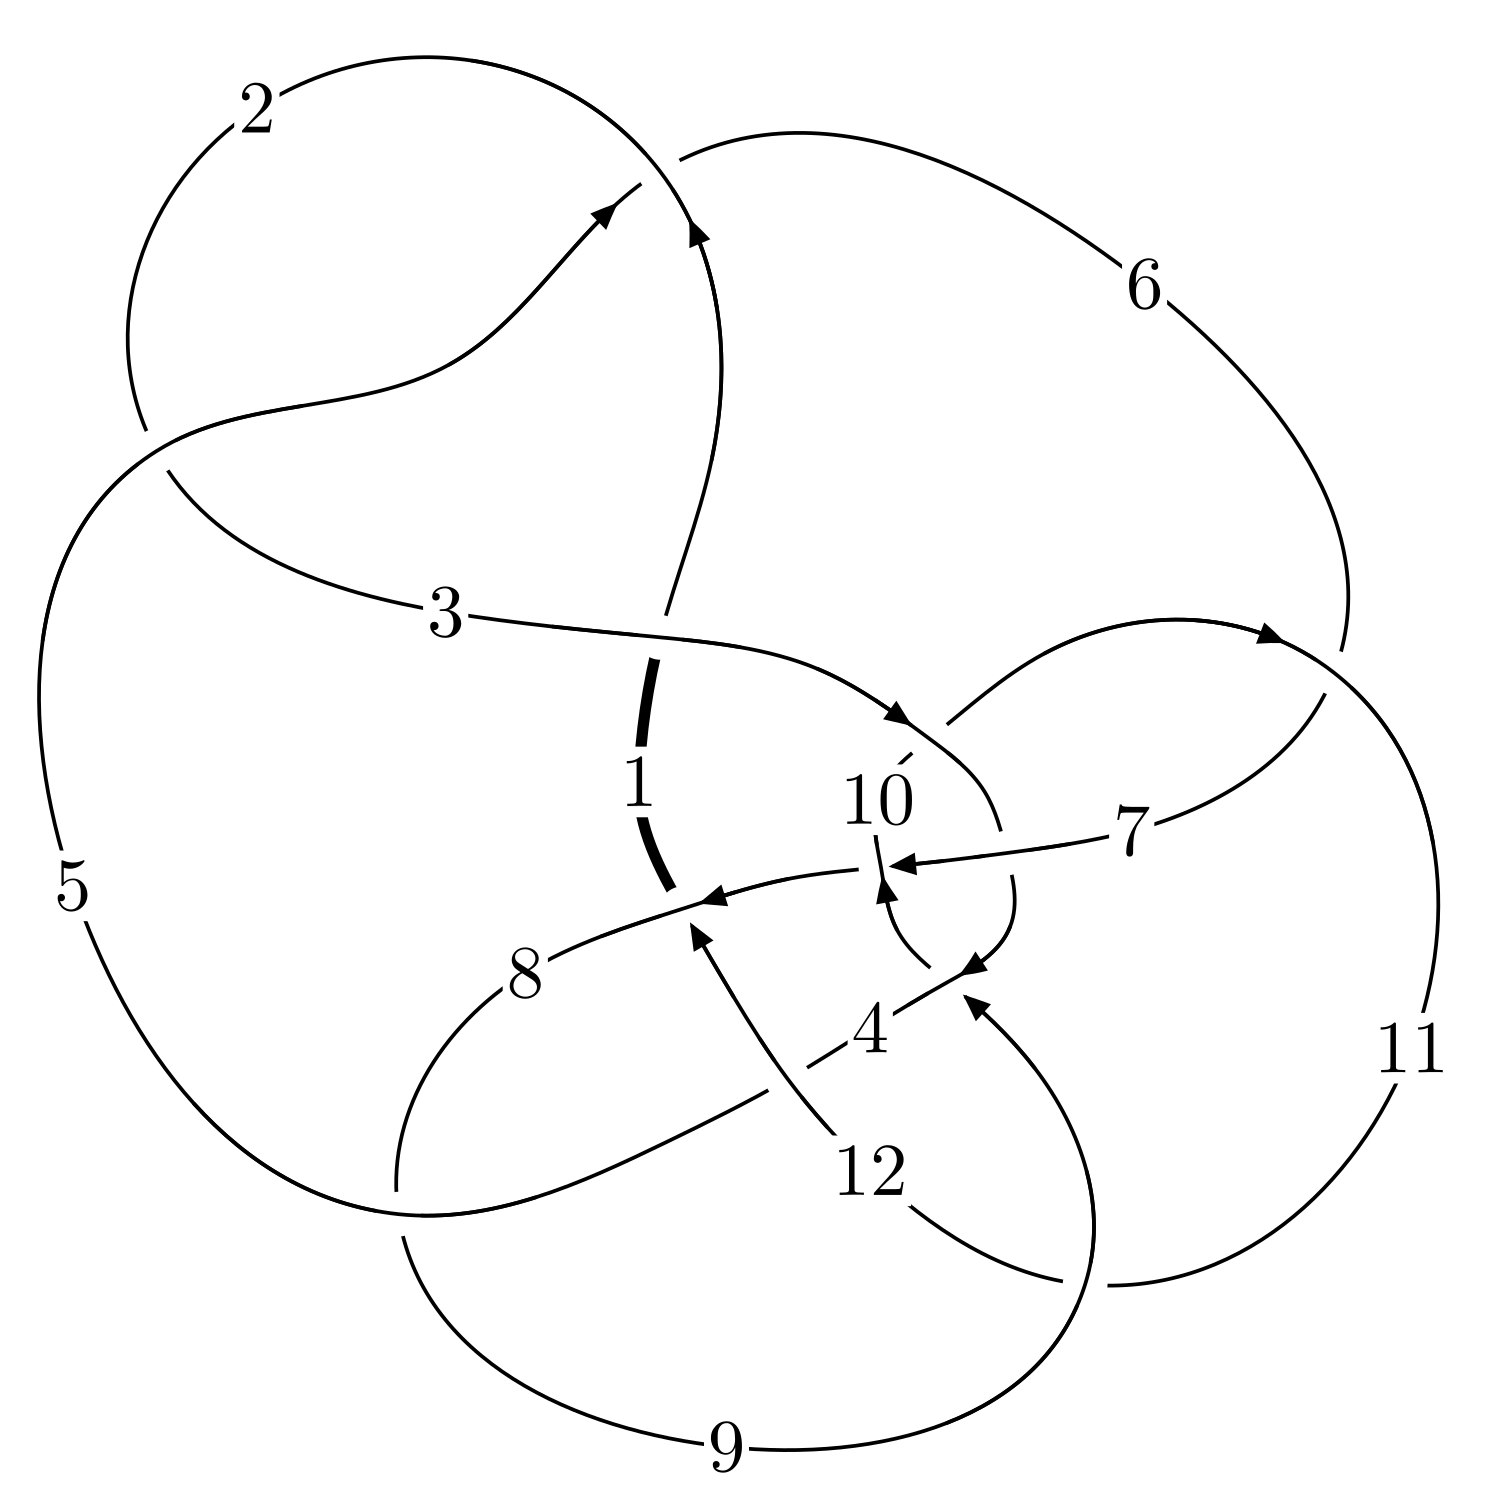
\includegraphics[width=112pt]{../../../GIT/diagram.site/Diagrams/png/2626_12n_0537.png}\\
\ \ \ A knot diagram\footnotemark}&
\allowdisplaybreaks
\textbf{Linearized knot diagam} \\
\cline{2-2}
 &
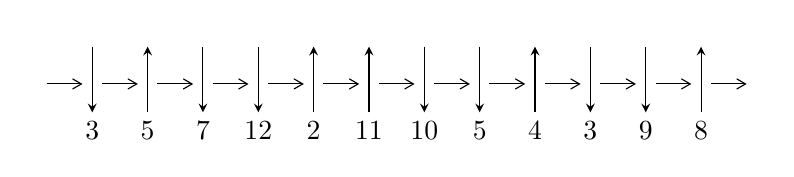
\begin{tikzpicture}[x=20pt, y=17pt]
	% nodes
	\node (C0) at (0, 0) {};
	\node (C1) at (1, 0) {};
	\node (C1U) at (1, +1) {};
	\node (C1D) at (1, -1) {3};

	\node (C2) at (2, 0) {};
	\node (C2U) at (2, +1) {};
	\node (C2D) at (2, -1) {5};

	\node (C3) at (3, 0) {};
	\node (C3U) at (3, +1) {};
	\node (C3D) at (3, -1) {7};

	\node (C4) at (4, 0) {};
	\node (C4U) at (4, +1) {};
	\node (C4D) at (4, -1) {12};

	\node (C5) at (5, 0) {};
	\node (C5U) at (5, +1) {};
	\node (C5D) at (5, -1) {2};

	\node (C6) at (6, 0) {};
	\node (C6U) at (6, +1) {};
	\node (C6D) at (6, -1) {11};

	\node (C7) at (7, 0) {};
	\node (C7U) at (7, +1) {};
	\node (C7D) at (7, -1) {10};

	\node (C8) at (8, 0) {};
	\node (C8U) at (8, +1) {};
	\node (C8D) at (8, -1) {5};

	\node (C9) at (9, 0) {};
	\node (C9U) at (9, +1) {};
	\node (C9D) at (9, -1) {4};

	\node (C10) at (10, 0) {};
	\node (C10U) at (10, +1) {};
	\node (C10D) at (10, -1) {3};

	\node (C11) at (11, 0) {};
	\node (C11U) at (11, +1) {};
	\node (C11D) at (11, -1) {9};

	\node (C12) at (12, 0) {};
	\node (C12U) at (12, +1) {};
	\node (C12D) at (12, -1) {8};
	\node (C13) at (13, 0) {};

	% arrows
	\draw[->,>={angle 60}]
	(C0) edge (C1) (C1) edge (C2) (C2) edge (C3) (C3) edge (C4) (C4) edge (C5) (C5) edge (C6) (C6) edge (C7) (C7) edge (C8) (C8) edge (C9) (C9) edge (C10) (C10) edge (C11) (C11) edge (C12) (C12) edge (C13) ;	\draw[->,>=stealth]
	(C1U) edge (C1D) (C2D) edge (C2U) (C3U) edge (C3D) (C4U) edge (C4D) (C5D) edge (C5U) (C6D) edge (C6U) (C7U) edge (C7D) (C8U) edge (C8D) (C9D) edge (C9U) (C10U) edge (C10D) (C11U) edge (C11D) (C12D) edge (C12U) ;
	\end{tikzpicture} \\
\hhline{~~} \\& 
\textbf{Solving Sequence} \\ \cline{2-2} 
 &
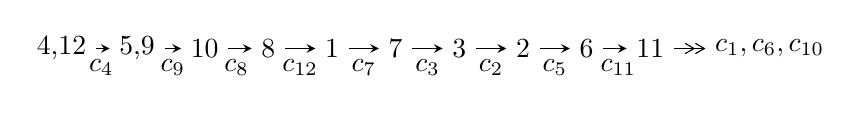
\begin{tikzpicture}[x=23pt, y=7pt]
	% node
	\node (A0) at (-1/8, 0) {4,12};
	\node (A1) at (17/16, 0) {5,9};
	\node (A2) at (17/8, 0) {10};
	\node (A3) at (25/8, 0) {8};
	\node (A4) at (33/8, 0) {1};
	\node (A5) at (41/8, 0) {7};
	\node (A6) at (49/8, 0) {3};
	\node (A7) at (57/8, 0) {2};
	\node (A8) at (65/8, 0) {6};
	\node (A9) at (73/8, 0) {11};
	\node (C1) at (1/2, -1) {$c_{4}$};
	\node (C2) at (13/8, -1) {$c_{9}$};
	\node (C3) at (21/8, -1) {$c_{8}$};
	\node (C4) at (29/8, -1) {$c_{12}$};
	\node (C5) at (37/8, -1) {$c_{7}$};
	\node (C6) at (45/8, -1) {$c_{3}$};
	\node (C7) at (53/8, -1) {$c_{2}$};
	\node (C8) at (61/8, -1) {$c_{5}$};
	\node (C9) at (69/8, -1) {$c_{11}$};
	\node (A10) at (11, 0) {$c_{1},c_{6},c_{10}$};

	% edge
	\draw[->,>=stealth]	
	(A0) edge (A1) (A1) edge (A2) (A2) edge (A3) (A3) edge (A4) (A4) edge (A5) (A5) edge (A6) (A6) edge (A7) (A7) edge (A8) (A8) edge (A9) ;
	\draw[->>,>={angle 60}]	
	(A9) edge (A10);
\end{tikzpicture} \\ 

\end{tabular} \\

\footnotetext{
The image of knot diagram is generated by the software ``\textbf{Draw programme}" developed by Andrew Bartholomew(\url{http://www.layer8.co.uk/maths/draw/index.htm\#Running-draw}), where we modified some parts for our purpose(\url{https://github.com/CATsTAILs/LinksPainter}).
}\phantom \\ \newline 
\centering \textbf{Ideals for irreducible components\footnotemark of $X_{\text{par}}$} 
 
\begin{align*}
I^u_{1}&=\langle 
-4.81893\times10^{17} u^{27}-6.03500\times10^{17} u^{26}+\cdots+5.35730\times10^{17} b-3.43509\times10^{18},\\
\phantom{I^u_{1}}&\phantom{= \langle  }-3.83926\times10^{18} u^{27}+2.85325\times10^{18} u^{26}+\cdots+5.35730\times10^{17} a-4.31215\times10^{18},\;u^{28}+2 u^{26}+\cdots+2 u+1\rangle \\
I^u_{2}&=\langle 
6.36861\times10^{214} u^{67}+1.23983\times10^{215} u^{66}+\cdots+2.21361\times10^{214} b+4.99066\times10^{215},\\
\phantom{I^u_{2}}&\phantom{= \langle  }-6.89986\times10^{215} u^{67}-1.24081\times10^{216} u^{66}+\cdots+2.21361\times10^{214} a-3.68206\times10^{216},\\
\phantom{I^u_{2}}&\phantom{= \langle  }u^{68}+2 u^{67}+\cdots+21 u+1\rangle \\
I^u_{3}&=\langle 
-2.25962\times10^{48} u^{35}-8.58758\times10^{47} u^{34}+\cdots+1.17942\times10^{46} b+5.94065\times10^{48},\\
\phantom{I^u_{3}}&\phantom{= \langle  }-1.61303\times10^{48} u^{35}-6.16039\times10^{47} u^{34}+\cdots+1.17942\times10^{46} a+4.20101\times10^{48},\;u^{36}+5 u^{34}+\cdots-6 u^2+1\rangle \\
I^u_{4}&=\langle 
b,\;2 u^4+u^3+3 u^2+a- u-2,\;u^5+u^3- u^2- u+1\rangle \\
I^u_{5}&=\langle 
b-1,\;a+1,\;u^2- u+1\rangle \\
\\
\end{align*}
\raggedright * 5 irreducible components of $\dim_{\mathbb{C}}=0$, with total 139 representations.\\
\footnotetext{All coefficients of polynomials are rational numbers. But the coefficients are sometimes approximated in decimal forms when there is not enough margin.}
\newpage
\renewcommand{\arraystretch}{1}
\centering \section*{I. $I^u_{1}= \langle -4.82\times10^{17} u^{27}-6.04\times10^{17} u^{26}+\cdots+5.36\times10^{17} b-3.44\times10^{18},\;-3.84\times10^{18} u^{27}+2.85\times10^{18} u^{26}+\cdots+5.36\times10^{17} a-4.31\times10^{18},\;u^{28}+2 u^{26}+\cdots+2 u+1 \rangle$}
\flushleft \textbf{(i) Arc colorings}\\
\begin{tabular}{m{7pt} m{180pt} m{7pt} m{180pt} }
\flushright $a_{4}=$&$\begin{pmatrix}1\\0\end{pmatrix}$ \\
\flushright $a_{12}=$&$\begin{pmatrix}0\\u\end{pmatrix}$ \\
\flushright $a_{5}=$&$\begin{pmatrix}1\\u^2\end{pmatrix}$ \\
\flushright $a_{9}=$&$\begin{pmatrix}7.16640 u^{27}-5.32591 u^{26}+\cdots+6.13836 u+8.04910\\0.899507 u^{27}+1.12650 u^{26}+\cdots+4.01358 u+6.41197\end{pmatrix}$ \\
\flushright $a_{10}=$&$\begin{pmatrix}8.06591 u^{27}-4.19941 u^{26}+\cdots+10.1519 u+14.4611\\0.899507 u^{27}+1.12650 u^{26}+\cdots+4.01358 u+6.41197\end{pmatrix}$ \\
\flushright $a_{8}=$&$\begin{pmatrix}5.18943 u^{27}-2.77194 u^{26}+\cdots+6.66653 u+9.13517\\0.163984 u^{27}+0.536152 u^{26}+\cdots+0.882630 u+3.85801\end{pmatrix}$ \\
\flushright $a_{1}=$&$\begin{pmatrix}6.83813 u^{27}-3.91955 u^{26}+\cdots+6.32359 u+12.0959\\-1.93722 u^{27}+1.48121 u^{26}+\cdots-1.00772 u-2.61673\end{pmatrix}$ \\
\flushright $a_{7}=$&$\begin{pmatrix}-14.1808 u^{27}+9.53294 u^{26}+\cdots-9.14159 u-22.3381\\u\end{pmatrix}$ \\
\flushright $a_{3}=$&$\begin{pmatrix}-9.53294 u^{27}+6.37147 u^{26}+\cdots-6.02353 u-13.1808\\- u^2\end{pmatrix}$ \\
\flushright $a_{2}=$&$\begin{pmatrix}-13.4897 u^{27}+8.98078 u^{26}+\cdots-9.23353 u-19.5523\\-1.82185 u^{27}+1.25415 u^{26}+\cdots-1.26190 u-2.60931\end{pmatrix}$ \\
\flushright $a_{6}=$&$\begin{pmatrix}5.48144 u^{27}-3.48713 u^{26}+\cdots+3.70672 u+8.83761\\1.93722 u^{27}-1.48121 u^{26}+\cdots+1.00772 u+2.61673\end{pmatrix}$ \\
\flushright $a_{11}=$&$\begin{pmatrix}19.2062 u^{27}-12.8410 u^{26}+\cdots+15.9255 u+27.6152\\0.163984 u^{27}+0.536152 u^{26}+\cdots+0.882630 u+3.85801\end{pmatrix}$\\&\end{tabular}
\flushleft \textbf{(ii) Obstruction class $= -1$}\\~\\
\flushleft \textbf{(iii) Cusp Shapes $= -\frac{18680269678576763267}{535729943333344787} u^{27}+\frac{8598753415343829290}{535729943333344787} u^{26}+\cdots-\frac{35223182169748815025}{535729943333344787} u-\frac{23029573736888830965}{535729943333344787}$}\\~\\
\newpage\renewcommand{\arraystretch}{1}
\flushleft \textbf{(iv) u-Polynomials at the component}\newline \\
\begin{tabular}{m{50pt}|m{274pt}}
Crossings & \hspace{64pt}u-Polynomials at each crossing \\
\hline $$\begin{aligned}c_{1}\end{aligned}$$&$\begin{aligned}
&u^{28}+27 u^{27}+\cdots+13748 u+1296
\end{aligned}$\\
\hline $$\begin{aligned}c_{2},c_{5}\end{aligned}$$&$\begin{aligned}
&u^{28}+3 u^{27}+\cdots+2 u+36
\end{aligned}$\\
\hline $$\begin{aligned}c_{3},c_{4}\end{aligned}$$&$\begin{aligned}
&u^{28}+2 u^{26}+\cdots+2 u+1
\end{aligned}$\\
\hline $$\begin{aligned}c_{6},c_{12}\end{aligned}$$&$\begin{aligned}
&u^{28}+8 u^{27}+\cdots+224 u+32
\end{aligned}$\\
\hline $$\begin{aligned}c_{7},c_{11}\end{aligned}$$&$\begin{aligned}
&u^{28}+3 u^{27}+\cdots+13 u+1
\end{aligned}$\\
\hline $$\begin{aligned}c_{8},c_{10}\end{aligned}$$&$\begin{aligned}
&u^{28}+u^{27}+\cdots-3 u+1
\end{aligned}$\\
\hline $$\begin{aligned}c_{9}\end{aligned}$$&$\begin{aligned}
&u^{28}+5 u^{27}+\cdots+320 u+128
\end{aligned}$\\
\hline
\end{tabular}\\~\\
\newpage\renewcommand{\arraystretch}{1}
\flushleft \textbf{(v) Riley Polynomials at the component}\newline \\
\begin{tabular}{m{50pt}|m{274pt}}
Crossings & \hspace{64pt}Riley Polynomials at each crossing \\
\hline $$\begin{aligned}c_{1}\end{aligned}$$&$\begin{aligned}
&y^{28}-49 y^{27}+\cdots-825712 y+1679616
\end{aligned}$\\
\hline $$\begin{aligned}c_{2},c_{5}\end{aligned}$$&$\begin{aligned}
&y^{28}+27 y^{27}+\cdots+13748 y+1296
\end{aligned}$\\
\hline $$\begin{aligned}c_{3},c_{4}\end{aligned}$$&$\begin{aligned}
&y^{28}+4 y^{27}+\cdots+6 y+1
\end{aligned}$\\
\hline $$\begin{aligned}c_{6},c_{12}\end{aligned}$$&$\begin{aligned}
&y^{28}+30 y^{27}+\cdots+29696 y+1024
\end{aligned}$\\
\hline $$\begin{aligned}c_{7},c_{11}\end{aligned}$$&$\begin{aligned}
&y^{28}- y^{27}+\cdots- y+1
\end{aligned}$\\
\hline $$\begin{aligned}c_{8},c_{10}\end{aligned}$$&$\begin{aligned}
&y^{28}-29 y^{27}+\cdots-45 y+1
\end{aligned}$\\
\hline $$\begin{aligned}c_{9}\end{aligned}$$&$\begin{aligned}
&y^{28}- y^{27}+\cdots+233472 y+16384
\end{aligned}$\\
\hline
\end{tabular}\\~\\
\newpage\flushleft \textbf{(vi) Complex Volumes and Cusp Shapes}
$$\begin{array}{c|c|c}  
\text{Solutions to }I^u_{1}& \I (\text{vol} + \sqrt{-1}CS) & \text{Cusp shape}\\
 \hline 
\begin{aligned}
u &= -0.668779 + 0.723827 I \\
a &= -1.042480 + 0.230333 I \\
b &= \phantom{-}0.533282 + 0.983247 I\end{aligned}
 & -0.10356 + 2.64453 I & \phantom{-}1.22282 - 3.18892 I \\ \hline\begin{aligned}
u &= -0.668779 - 0.723827 I \\
a &= -1.042480 - 0.230333 I \\
b &= \phantom{-}0.533282 - 0.983247 I\end{aligned}
 & -0.10356 - 2.64453 I & \phantom{-}1.22282 + 3.18892 I \\ \hline\begin{aligned}
u &= \phantom{-}0.635506 + 0.698040 I \\
a &= \phantom{-}1.370710 + 0.155616 I \\
b &= -2.42228 - 0.22270 I\end{aligned}
 & -8.72712 - 8.29781 I & -3.70457 + 10.88184 I \\ \hline\begin{aligned}
u &= \phantom{-}0.635506 - 0.698040 I \\
a &= \phantom{-}1.370710 - 0.155616 I \\
b &= -2.42228 + 0.22270 I\end{aligned}
 & -8.72712 + 8.29781 I & -3.70457 - 10.88184 I \\ \hline\begin{aligned}
u &= \phantom{-}0.048408 + 0.902686 I \\
a &= \phantom{-}1.55642 - 0.39395 I \\
b &= -0.456492 + 0.690736 I\end{aligned}
 & -6.94969 - 1.95373 I & \phantom{-}0.13138 + 3.39783 I \\ \hline\begin{aligned}
u &= \phantom{-}0.048408 - 0.902686 I \\
a &= \phantom{-}1.55642 + 0.39395 I \\
b &= -0.456492 - 0.690736 I\end{aligned}
 & -6.94969 + 1.95373 I & \phantom{-}0.13138 - 3.39783 I \\ \hline\begin{aligned}
u &= \phantom{-}0.983916 + 0.634599 I \\
a &= \phantom{-}0.837957 + 0.541891 I \\
b &= -0.560930 + 1.151500 I\end{aligned}
 & -2.43111 - 6.54317 I & -6.80530 + 6.55208 I \\ \hline\begin{aligned}
u &= \phantom{-}0.983916 - 0.634599 I \\
a &= \phantom{-}0.837957 - 0.541891 I \\
b &= -0.560930 - 1.151500 I\end{aligned}
 & -2.43111 + 6.54317 I & -6.80530 - 6.55208 I \\ \hline\begin{aligned}
u &= -0.278802 + 0.692018 I \\
a &= -1.019280 - 0.484379 I \\
b &= \phantom{-}2.06902 + 0.53469 I\end{aligned}
 & -0.15480 + 3.78570 I & \phantom{-}3.46312 - 12.68951 I \\ \hline\begin{aligned}
u &= -0.278802 - 0.692018 I \\
a &= -1.019280 + 0.484379 I \\
b &= \phantom{-}2.06902 - 0.53469 I\end{aligned}
 & -0.15480 - 3.78570 I & \phantom{-}3.46312 + 12.68951 I\\
 \hline 
 \end{array}$$\newpage$$\begin{array}{c|c|c}  
\text{Solutions to }I^u_{1}& \I (\text{vol} + \sqrt{-1}CS) & \text{Cusp shape}\\
 \hline 
\begin{aligned}
u &= -0.262782 + 0.616933 I \\
a &= \phantom{-}0.103884 - 0.340572 I \\
b &= -0.836041 + 0.476997 I\end{aligned}
 & \phantom{-}0.01742 + 1.41732 I & -1.09305 - 2.14471 I \\ \hline\begin{aligned}
u &= -0.262782 - 0.616933 I \\
a &= \phantom{-}0.103884 + 0.340572 I \\
b &= -0.836041 - 0.476997 I\end{aligned}
 & \phantom{-}0.01742 - 1.41732 I & -1.09305 + 2.14471 I \\ \hline\begin{aligned}
u &= -0.659524 + 0.003319 I \\
a &= -2.13553 + 2.39966 I \\
b &= \phantom{-}0.278963 + 0.671140 I\end{aligned}
 & -9.47298 + 2.59610 I & -14.8510 - 6.7959 I \\ \hline\begin{aligned}
u &= -0.659524 - 0.003319 I \\
a &= -2.13553 - 2.39966 I \\
b &= \phantom{-}0.278963 - 0.671140 I\end{aligned}
 & -9.47298 - 2.59610 I & -14.8510 + 6.7959 I \\ \hline\begin{aligned}
u &= \phantom{-}0.572072 + 0.249132 I \\
a &= \phantom{-}2.09983 + 0.65588 I \\
b &= -0.562847 + 0.942357 I\end{aligned}
 & -2.94382 - 1.92479 I & -11.20798 + 2.16356 I \\ \hline\begin{aligned}
u &= \phantom{-}0.572072 - 0.249132 I \\
a &= \phantom{-}2.09983 - 0.65588 I \\
b &= -0.562847 - 0.942357 I\end{aligned}
 & -2.94382 + 1.92479 I & -11.20798 - 2.16356 I \\ \hline\begin{aligned}
u &= -0.163734 + 0.512554 I \\
a &= -0.561467 - 0.153031 I \\
b &= -0.152593 + 0.805696 I\end{aligned}
 & \phantom{-}0.027219 + 1.275630 I & \phantom{-}0.54017 - 5.75782 I \\ \hline\begin{aligned}
u &= -0.163734 - 0.512554 I \\
a &= -0.561467 + 0.153031 I \\
b &= -0.152593 - 0.805696 I\end{aligned}
 & \phantom{-}0.027219 - 1.275630 I & \phantom{-}0.54017 + 5.75782 I \\ \hline\begin{aligned}
u &= -0.20976 + 1.48222 I \\
a &= -0.275606 - 0.434449 I \\
b &= \phantom{-}0.209091 + 0.559595 I\end{aligned}
 & \phantom{-}2.42708 + 1.71113 I & -8.50690 - 8.37300 I \\ \hline\begin{aligned}
u &= -0.20976 - 1.48222 I \\
a &= -0.275606 + 0.434449 I \\
b &= \phantom{-}0.209091 - 0.559595 I\end{aligned}
 & \phantom{-}2.42708 - 1.71113 I & -8.50690 + 8.37300 I\\
 \hline 
 \end{array}$$\newpage$$\begin{array}{c|c|c}  
\text{Solutions to }I^u_{1}& \I (\text{vol} + \sqrt{-1}CS) & \text{Cusp shape}\\
 \hline 
\begin{aligned}
u &= -1.15979 + 1.04033 I \\
a &= \phantom{-}1.179480 + 0.124327 I \\
b &= -0.87720 - 1.53540 I\end{aligned}
 & -12.9356 + 18.0876 I & -5.50986 - 8.24727 I \\ \hline\begin{aligned}
u &= -1.15979 - 1.04033 I \\
a &= \phantom{-}1.179480 - 0.124327 I \\
b &= -0.87720 + 1.53540 I\end{aligned}
 & -12.9356 - 18.0876 I & -5.50986 + 8.24727 I \\ \hline\begin{aligned}
u &= \phantom{-}1.14462 + 1.07762 I \\
a &= -0.343283 + 0.540527 I \\
b &= \phantom{-}0.060499 - 1.217480 I\end{aligned}
 & -12.42660 + 1.51018 I & -8.64520 + 0. I\phantom{ +0.000000I} \\ \hline\begin{aligned}
u &= \phantom{-}1.14462 - 1.07762 I \\
a &= -0.343283 - 0.540527 I \\
b &= \phantom{-}0.060499 + 1.217480 I\end{aligned}
 & -12.42660 - 1.51018 I & -8.64520 + 0. I\phantom{ +0.000000I} \\ \hline\begin{aligned}
u &= -1.15228 + 1.07906 I \\
a &= \phantom{-}0.632964 + 0.320798 I \\
b &= -0.526893 - 1.288980 I\end{aligned}
 & -4.70997 + 4.71020 I & -6.97281 - 3.71311 I \\ \hline\begin{aligned}
u &= -1.15228 - 1.07906 I \\
a &= \phantom{-}0.632964 - 0.320798 I \\
b &= -0.526893 + 1.288980 I\end{aligned}
 & -4.70997 - 4.71020 I & -6.97281 + 3.71311 I \\ \hline\begin{aligned}
u &= \phantom{-}1.17094 + 1.06658 I \\
a &= -0.903598 + 0.197693 I \\
b &= \phantom{-}0.74443 - 1.44446 I\end{aligned}
 & -4.94640 - 12.28330 I & -5.06082 + 8.01009 I \\ \hline\begin{aligned}
u &= \phantom{-}1.17094 - 1.06658 I \\
a &= -0.903598 - 0.197693 I \\
b &= \phantom{-}0.74443 + 1.44446 I\end{aligned}
 & -4.94640 + 12.28330 I & -5.06082 - 8.01009 I\\
 \hline 
 \end{array}$$\newpage\newpage\renewcommand{\arraystretch}{1}
\centering \section*{II. $I^u_{2}= \langle 6.37\times10^{214} u^{67}+1.24\times10^{215} u^{66}+\cdots+2.21\times10^{214} b+4.99\times10^{215},\;-6.90\times10^{215} u^{67}-1.24\times10^{216} u^{66}+\cdots+2.21\times10^{214} a-3.68\times10^{216},\;u^{68}+2 u^{67}+\cdots+21 u+1 \rangle$}
\flushleft \textbf{(i) Arc colorings}\\
\begin{tabular}{m{7pt} m{180pt} m{7pt} m{180pt} }
\flushright $a_{4}=$&$\begin{pmatrix}1\\0\end{pmatrix}$ \\
\flushright $a_{12}=$&$\begin{pmatrix}0\\u\end{pmatrix}$ \\
\flushright $a_{5}=$&$\begin{pmatrix}1\\u^2\end{pmatrix}$ \\
\flushright $a_{9}=$&$\begin{pmatrix}31.1702 u^{67}+56.0539 u^{66}+\cdots+2647.88 u+166.338\\-2.87703 u^{67}-5.60095 u^{66}+\cdots-328.693 u-22.5454\end{pmatrix}$ \\
\flushright $a_{10}=$&$\begin{pmatrix}28.2932 u^{67}+50.4529 u^{66}+\cdots+2319.19 u+143.792\\-2.87703 u^{67}-5.60095 u^{66}+\cdots-328.693 u-22.5454\end{pmatrix}$ \\
\flushright $a_{8}=$&$\begin{pmatrix}26.7127 u^{67}+47.8406 u^{66}+\cdots+2218.34 u+137.506\\-2.95446 u^{67}-5.72854 u^{66}+\cdots-338.974 u-23.2473\end{pmatrix}$ \\
\flushright $a_{1}=$&$\begin{pmatrix}88.0011 u^{67}+162.387 u^{66}+\cdots+8091.09 u+542.171\\-5.68870 u^{67}-10.3246 u^{66}+\cdots-569.445 u-41.1034\end{pmatrix}$ \\
\flushright $a_{7}=$&$\begin{pmatrix}5.00717 u^{67}+8.61197 u^{66}+\cdots+214.047 u-9.36045\\-3.79980 u^{67}-7.12911 u^{66}+\cdots-372.019 u-24.6242\end{pmatrix}$ \\
\flushright $a_{3}=$&$\begin{pmatrix}-63.6091 u^{67}-117.431 u^{66}+\cdots-5857.97 u-389.038\\4.84840 u^{67}+8.68921 u^{66}+\cdots+432.644 u+30.6341\end{pmatrix}$ \\
\flushright $a_{2}=$&$\begin{pmatrix}-69.4105 u^{67}-128.375 u^{66}+\cdots-6432.53 u-429.459\\4.85010 u^{67}+8.61831 u^{66}+\cdots+424.612 u+29.9753\end{pmatrix}$ \\
\flushright $a_{6}=$&$\begin{pmatrix}-63.3932 u^{67}-117.128 u^{66}+\cdots-6447.05 u-489.180\\-3.77612 u^{67}-6.57578 u^{66}+\cdots-244.295 u-13.6639\end{pmatrix}$ \\
\flushright $a_{11}=$&$\begin{pmatrix}102.661 u^{67}+190.241 u^{66}+\cdots+9665.96 u+654.485\\-5.94412 u^{67}-11.0219 u^{66}+\cdots-591.464 u-42.5143\end{pmatrix}$\\&\end{tabular}
\flushleft \textbf{(ii) Obstruction class $= -1$}\\~\\
\flushleft \textbf{(iii) Cusp Shapes $= 0.381385 u^{67}+4.09349 u^{66}+\cdots+460.637 u+29.8348$}\\~\\
\newpage\renewcommand{\arraystretch}{1}
\flushleft \textbf{(iv) u-Polynomials at the component}\newline \\
\begin{tabular}{m{50pt}|m{274pt}}
Crossings & \hspace{64pt}u-Polynomials at each crossing \\
\hline $$\begin{aligned}c_{1}\end{aligned}$$&$\begin{aligned}
&(u^{34}+44 u^{33}+\cdots+211167 u+11664)^{2}
\end{aligned}$\\
\hline $$\begin{aligned}c_{2},c_{5}\end{aligned}$$&$\begin{aligned}
&(u^{34}-2 u^{33}+\cdots-27 u+108)^{2}
\end{aligned}$\\
\hline $$\begin{aligned}c_{3},c_{4}\end{aligned}$$&$\begin{aligned}
&u^{68}+2 u^{67}+\cdots+21 u+1
\end{aligned}$\\
\hline $$\begin{aligned}c_{6},c_{12}\end{aligned}$$&$\begin{aligned}
&u^{68}-6 u^{67}+\cdots+218203862 u+59673407
\end{aligned}$\\
\hline $$\begin{aligned}c_{7},c_{11}\end{aligned}$$&$\begin{aligned}
&u^{68}+3 u^{67}+\cdots+311 u+59
\end{aligned}$\\
\hline $$\begin{aligned}c_{8},c_{10}\end{aligned}$$&$\begin{aligned}
&u^{68}+u^{67}+\cdots+927119 u+1344671
\end{aligned}$\\
\hline $$\begin{aligned}c_{9}\end{aligned}$$&$\begin{aligned}
&(u^{34}- u^{33}+\cdots-71 u+209)^{2}
\end{aligned}$\\
\hline
\end{tabular}\\~\\
\newpage\renewcommand{\arraystretch}{1}
\flushleft \textbf{(v) Riley Polynomials at the component}\newline \\
\begin{tabular}{m{50pt}|m{274pt}}
Crossings & \hspace{64pt}Riley Polynomials at each crossing \\
\hline $$\begin{aligned}c_{1}\end{aligned}$$&$\begin{aligned}
&(y^{34}-92 y^{33}+\cdots+1741335327 y+136048896)^{2}
\end{aligned}$\\
\hline $$\begin{aligned}c_{2},c_{5}\end{aligned}$$&$\begin{aligned}
&(y^{34}+44 y^{33}+\cdots+211167 y+11664)^{2}
\end{aligned}$\\
\hline $$\begin{aligned}c_{3},c_{4}\end{aligned}$$&$\begin{aligned}
&y^{68}-2 y^{67}+\cdots-119 y+1
\end{aligned}$\\
\hline $$\begin{aligned}c_{6},c_{12}\end{aligned}$$&$\begin{aligned}
&y^{68}+24 y^{67}+\cdots+109187012423296144 y+3560915502987649
\end{aligned}$\\
\hline $$\begin{aligned}c_{7},c_{11}\end{aligned}$$&$\begin{aligned}
&y^{68}-35 y^{67}+\cdots+19745 y+3481
\end{aligned}$\\
\hline $$\begin{aligned}c_{8},c_{10}\end{aligned}$$&$\begin{aligned}
&y^{68}-13 y^{67}+\cdots-6278009008341 y+1808140098241
\end{aligned}$\\
\hline $$\begin{aligned}c_{9}\end{aligned}$$&$\begin{aligned}
&(y^{34}+27 y^{33}+\cdots+812985 y+43681)^{2}
\end{aligned}$\\
\hline
\end{tabular}\\~\\
\newpage\flushleft \textbf{(vi) Complex Volumes and Cusp Shapes}
$$\begin{array}{c|c|c}  
\text{Solutions to }I^u_{2}& \I (\text{vol} + \sqrt{-1}CS) & \text{Cusp shape}\\
 \hline 
\begin{aligned}
u &= -0.988229 + 0.036641 I \\
a &= \phantom{-}0.541719 - 0.076017 I \\
b &= -0.092881 + 0.993847 I\end{aligned}
 & -2.68708 + 3.24701 I & -7.49713 - 2.56448 I \\ \hline\begin{aligned}
u &= -0.988229 - 0.036641 I \\
a &= \phantom{-}0.541719 + 0.076017 I \\
b &= -0.092881 - 0.993847 I\end{aligned}
 & -2.68708 - 3.24701 I & -7.49713 + 2.56448 I \\ \hline\begin{aligned}
u &= \phantom{-}1.048190 + 0.084796 I \\
a &= -0.740063 + 0.401409 I \\
b &= \phantom{-}0.74542 - 1.31472 I\end{aligned}
 & -11.74950 + 0.99052 I & \phantom{-0.000000 } 0 \\ \hline\begin{aligned}
u &= \phantom{-}1.048190 - 0.084796 I \\
a &= -0.740063 - 0.401409 I \\
b &= \phantom{-}0.74542 + 1.31472 I\end{aligned}
 & -11.74950 - 0.99052 I & \phantom{-0.000000 } 0 \\ \hline\begin{aligned}
u &= \phantom{-}0.897611 + 0.299654 I \\
a &= \phantom{-}0.81753 - 2.31884 I \\
b &= \phantom{-}0.899935 - 0.657412 I\end{aligned}
 & -10.05820 + 4.24924 I & -11.45347 - 2.51859 I \\ \hline\begin{aligned}
u &= \phantom{-}0.897611 - 0.299654 I \\
a &= \phantom{-}0.81753 + 2.31884 I \\
b &= \phantom{-}0.899935 + 0.657412 I\end{aligned}
 & -10.05820 - 4.24924 I & -11.45347 + 2.51859 I \\ \hline\begin{aligned}
u &= \phantom{-}0.316205 + 1.016990 I \\
a &= -1.18839 + 1.71559 I \\
b &= \phantom{-}0.263043 - 1.081580 I\end{aligned}
 & -7.73519 - 5.04941 I & \phantom{-0.000000 } 0 \\ \hline\begin{aligned}
u &= \phantom{-}0.316205 - 1.016990 I \\
a &= -1.18839 - 1.71559 I \\
b &= \phantom{-}0.263043 + 1.081580 I\end{aligned}
 & -7.73519 + 5.04941 I & \phantom{-0.000000 } 0 \\ \hline\begin{aligned}
u &= \phantom{-}0.685355 + 0.849666 I \\
a &= \phantom{-}0.268449 + 0.431117 I \\
b &= \phantom{-}0.223062 + 0.797775 I\end{aligned}
 & -6.57994 - 2.99755 I & \phantom{-0.000000 } 0 \\ \hline\begin{aligned}
u &= \phantom{-}0.685355 - 0.849666 I \\
a &= \phantom{-}0.268449 - 0.431117 I \\
b &= \phantom{-}0.223062 - 0.797775 I\end{aligned}
 & -6.57994 + 2.99755 I & \phantom{-0.000000 } 0\\
 \hline 
 \end{array}$$\newpage$$\begin{array}{c|c|c}  
\text{Solutions to }I^u_{2}& \I (\text{vol} + \sqrt{-1}CS) & \text{Cusp shape}\\
 \hline 
\begin{aligned}
u &= -0.468927 + 0.753341 I \\
a &= \phantom{-}1.82075 + 0.71765 I \\
b &= -0.601383 - 0.937913 I\end{aligned}
 & \phantom{-}0.30115 + 6.48305 I & \phantom{-}2.75382 - 11.37072 I \\ \hline\begin{aligned}
u &= -0.468927 - 0.753341 I \\
a &= \phantom{-}1.82075 - 0.71765 I \\
b &= -0.601383 + 0.937913 I\end{aligned}
 & \phantom{-}0.30115 - 6.48305 I & \phantom{-}2.75382 + 11.37072 I \\ \hline\begin{aligned}
u &= -0.247431 + 0.841447 I \\
a &= -0.006812 - 0.392523 I \\
b &= -0.608249 + 1.119590 I\end{aligned}
 & \phantom{-}0.134730 + 1.289890 I & \phantom{-}2.62841 - 5.51442 I \\ \hline\begin{aligned}
u &= -0.247431 - 0.841447 I \\
a &= -0.006812 + 0.392523 I \\
b &= -0.608249 - 1.119590 I\end{aligned}
 & \phantom{-}0.134730 - 1.289890 I & \phantom{-}2.62841 + 5.51442 I \\ \hline\begin{aligned}
u &= -0.799604 + 0.350430 I \\
a &= -1.359860 - 0.075744 I \\
b &= \phantom{-}0.899935 - 0.657412 I\end{aligned}
 & -10.05820 + 4.24924 I & -11.45347 - 2.51859 I \\ \hline\begin{aligned}
u &= -0.799604 - 0.350430 I \\
a &= -1.359860 + 0.075744 I \\
b &= \phantom{-}0.899935 + 0.657412 I\end{aligned}
 & -10.05820 - 4.24924 I & -11.45347 + 2.51859 I \\ \hline\begin{aligned}
u &= -0.863696 + 0.007111 I \\
a &= -1.55464 + 0.90908 I \\
b &= -0.360465 + 0.686126 I\end{aligned}
 & -3.46175 + 1.42507 I & -10.51067 - 4.72604 I \\ \hline\begin{aligned}
u &= -0.863696 - 0.007111 I \\
a &= -1.55464 - 0.90908 I \\
b &= -0.360465 - 0.686126 I\end{aligned}
 & -3.46175 - 1.42507 I & -10.51067 + 4.72604 I \\ \hline\begin{aligned}
u &= -0.790910 + 0.123927 I \\
a &= \phantom{-}1.041290 + 0.463826 I \\
b &= -1.26373 - 1.89895 I\end{aligned}
 & -12.11020 + 6.39851 I & -11.48496 - 5.28007 I \\ \hline\begin{aligned}
u &= -0.790910 - 0.123927 I \\
a &= \phantom{-}1.041290 - 0.463826 I \\
b &= -1.26373 + 1.89895 I\end{aligned}
 & -12.11020 - 6.39851 I & -11.48496 + 5.28007 I\\
 \hline 
 \end{array}$$\newpage$$\begin{array}{c|c|c}  
\text{Solutions to }I^u_{2}& \I (\text{vol} + \sqrt{-1}CS) & \text{Cusp shape}\\
 \hline 
\begin{aligned}
u &= \phantom{-}0.744234 + 0.181720 I \\
a &= -0.77241 + 1.52342 I \\
b &= -0.404490 + 0.921778 I\end{aligned}
 & -2.66841 - 5.52402 I & -9.8516 + 10.9069 I \\ \hline\begin{aligned}
u &= \phantom{-}0.744234 - 0.181720 I \\
a &= -0.77241 - 1.52342 I \\
b &= -0.404490 - 0.921778 I\end{aligned}
 & -2.66841 + 5.52402 I & -9.8516 - 10.9069 I \\ \hline\begin{aligned}
u &= -0.139920 + 1.247210 I \\
a &= \phantom{-}0.063353 + 1.141210 I \\
b &= \phantom{-}0.059202 - 0.623325 I\end{aligned}
 & \phantom{-}4.42322 + 2.94331 I & \phantom{-0.000000 } 0 \\ \hline\begin{aligned}
u &= -0.139920 - 1.247210 I \\
a &= \phantom{-}0.063353 - 1.141210 I \\
b &= \phantom{-}0.059202 + 0.623325 I\end{aligned}
 & \phantom{-}4.42322 - 2.94331 I & \phantom{-0.000000 } 0 \\ \hline\begin{aligned}
u &= \phantom{-}1.089210 + 0.651528 I \\
a &= \phantom{-}1.127320 + 0.267005 I \\
b &= -0.404490 + 0.921778 I\end{aligned}
 & -2.66841 - 5.52402 I & \phantom{-0.000000 } 0 \\ \hline\begin{aligned}
u &= \phantom{-}1.089210 - 0.651528 I \\
a &= \phantom{-}1.127320 - 0.267005 I \\
b &= -0.404490 - 0.921778 I\end{aligned}
 & -2.66841 + 5.52402 I & \phantom{-0.000000 } 0 \\ \hline\begin{aligned}
u &= \phantom{-}0.559625 + 0.428522 I \\
a &= -1.65845 - 0.12542 I \\
b &= \phantom{-}0.86109 - 1.26732 I\end{aligned}
 & -1.33870 - 6.60010 I & -6.29119 + 6.93498 I \\ \hline\begin{aligned}
u &= \phantom{-}0.559625 - 0.428522 I \\
a &= -1.65845 + 0.12542 I \\
b &= \phantom{-}0.86109 + 1.26732 I\end{aligned}
 & -1.33870 + 6.60010 I & -6.29119 - 6.93498 I \\ \hline\begin{aligned}
u &= -0.641696 + 1.127080 I \\
a &= \phantom{-}0.464741 - 0.402605 I \\
b &= -1.078840 + 0.695928 I\end{aligned}
 & \phantom{-}0.362177 + 0.737675 I & \phantom{-0.000000 } 0 \\ \hline\begin{aligned}
u &= -0.641696 - 1.127080 I \\
a &= \phantom{-}0.464741 + 0.402605 I \\
b &= -1.078840 - 0.695928 I\end{aligned}
 & \phantom{-}0.362177 - 0.737675 I & \phantom{-0.000000 } 0\\
 \hline 
 \end{array}$$\newpage$$\begin{array}{c|c|c}  
\text{Solutions to }I^u_{2}& \I (\text{vol} + \sqrt{-1}CS) & \text{Cusp shape}\\
 \hline 
\begin{aligned}
u &= \phantom{-}0.692090 + 0.104185 I \\
a &= \phantom{-}1.62625 - 0.34239 I \\
b &= -0.360465 - 0.686126 I\end{aligned}
 & -3.46175 - 1.42507 I & -10.51067 + 4.72604 I \\ \hline\begin{aligned}
u &= \phantom{-}0.692090 - 0.104185 I \\
a &= \phantom{-}1.62625 + 0.34239 I \\
b &= -0.360465 + 0.686126 I\end{aligned}
 & -3.46175 + 1.42507 I & -10.51067 - 4.72604 I \\ \hline\begin{aligned}
u &= -0.630362 + 1.147050 I \\
a &= -0.606718 - 0.469413 I \\
b &= \phantom{-}0.89698 + 1.81746 I\end{aligned}
 & -1.23903 + 3.47975 I & \phantom{-0.000000 } 0 \\ \hline\begin{aligned}
u &= -0.630362 - 1.147050 I \\
a &= -0.606718 + 0.469413 I \\
b &= \phantom{-}0.89698 - 1.81746 I\end{aligned}
 & -1.23903 - 3.47975 I & \phantom{-0.000000 } 0 \\ \hline\begin{aligned}
u &= -1.214430 + 0.596977 I \\
a &= -1.203930 + 0.263018 I \\
b &= \phantom{-}0.624993 + 0.841916 I\end{aligned}
 & -10.68940 + 6.84316 I & \phantom{-0.000000 } 0 \\ \hline\begin{aligned}
u &= -1.214430 - 0.596977 I \\
a &= -1.203930 - 0.263018 I \\
b &= \phantom{-}0.624993 - 0.841916 I\end{aligned}
 & -10.68940 - 6.84316 I & \phantom{-0.000000 } 0 \\ \hline\begin{aligned}
u &= -1.055410 + 0.872464 I \\
a &= -0.935528 - 0.245342 I \\
b &= -0.092881 + 0.993847 I\end{aligned}
 & -2.68708 + 3.24701 I & \phantom{-0.000000 } 0 \\ \hline\begin{aligned}
u &= -1.055410 - 0.872464 I \\
a &= -0.935528 + 0.245342 I \\
b &= -0.092881 - 0.993847 I\end{aligned}
 & -2.68708 - 3.24701 I & \phantom{-0.000000 } 0 \\ \hline\begin{aligned}
u &= -0.505178 + 0.289459 I \\
a &= \phantom{-}1.303920 - 0.401547 I \\
b &= -1.078840 - 0.695928 I\end{aligned}
 & \phantom{-}0.362177 - 0.737675 I & -3.01494 - 2.57610 I \\ \hline\begin{aligned}
u &= -0.505178 - 0.289459 I \\
a &= \phantom{-}1.303920 + 0.401547 I \\
b &= -1.078840 + 0.695928 I\end{aligned}
 & \phantom{-}0.362177 + 0.737675 I & -3.01494 + 2.57610 I\\
 \hline 
 \end{array}$$\newpage$$\begin{array}{c|c|c}  
\text{Solutions to }I^u_{2}& \I (\text{vol} + \sqrt{-1}CS) & \text{Cusp shape}\\
 \hline 
\begin{aligned}
u &= \phantom{-}1.03822 + 0.97416 I \\
a &= \phantom{-}1.292760 - 0.248045 I \\
b &= -1.26373 + 1.89895 I\end{aligned}
 & -12.11020 - 6.39851 I & \phantom{-0.000000 } 0 \\ \hline\begin{aligned}
u &= \phantom{-}1.03822 - 0.97416 I \\
a &= \phantom{-}1.292760 + 0.248045 I \\
b &= -1.26373 - 1.89895 I\end{aligned}
 & -12.11020 + 6.39851 I & \phantom{-0.000000 } 0 \\ \hline\begin{aligned}
u &= \phantom{-}0.95320 + 1.07772 I \\
a &= \phantom{-}0.470263 - 1.062870 I \\
b &= \phantom{-}0.74542 + 1.31472 I\end{aligned}
 & -11.74950 - 0.99052 I & \phantom{-0.000000 } 0 \\ \hline\begin{aligned}
u &= \phantom{-}0.95320 - 1.07772 I \\
a &= \phantom{-}0.470263 + 1.062870 I \\
b &= \phantom{-}0.74542 - 1.31472 I\end{aligned}
 & -11.74950 + 0.99052 I & \phantom{-0.000000 } 0 \\ \hline\begin{aligned}
u &= \phantom{-}0.541931 + 0.113704 I \\
a &= -0.169744 - 0.186828 I \\
b &= \phantom{-}0.89698 + 1.81746 I\end{aligned}
 & -1.23903 + 3.47975 I & -11.86128 + 7.58185 I \\ \hline\begin{aligned}
u &= \phantom{-}0.541931 - 0.113704 I \\
a &= -0.169744 + 0.186828 I \\
b &= \phantom{-}0.89698 - 1.81746 I\end{aligned}
 & -1.23903 - 3.47975 I & -11.86128 - 7.58185 I \\ \hline\begin{aligned}
u &= -0.486109 + 0.250377 I \\
a &= \phantom{-}0.54394 + 5.66734 I \\
b &= \phantom{-}0.624993 + 0.841916 I\end{aligned}
 & -10.68940 + 6.84316 I & -13.1700 - 13.6418 I \\ \hline\begin{aligned}
u &= -0.486109 - 0.250377 I \\
a &= \phantom{-}0.54394 - 5.66734 I \\
b &= \phantom{-}0.624993 - 0.841916 I\end{aligned}
 & -10.68940 - 6.84316 I & -13.1700 + 13.6418 I \\ \hline\begin{aligned}
u &= -1.20413 + 0.91553 I \\
a &= -0.977470 + 0.362937 I \\
b &= \phantom{-}0.86109 + 1.26732 I\end{aligned}
 & -1.33870 + 6.60010 I & \phantom{-0.000000 } 0 \\ \hline\begin{aligned}
u &= -1.20413 - 0.91553 I \\
a &= -0.977470 - 0.362937 I \\
b &= \phantom{-}0.86109 - 1.26732 I\end{aligned}
 & -1.33870 - 6.60010 I & \phantom{-0.000000 } 0\\
 \hline 
 \end{array}$$\newpage$$\begin{array}{c|c|c}  
\text{Solutions to }I^u_{2}& \I (\text{vol} + \sqrt{-1}CS) & \text{Cusp shape}\\
 \hline 
\begin{aligned}
u &= \phantom{-}1.10477 + 1.07329 I \\
a &= -1.038600 + 0.326925 I \\
b &= \phantom{-}0.543096 - 1.209800 I\end{aligned}
 & -12.3962 - 9.6578 I & \phantom{-0.000000 } 0 \\ \hline\begin{aligned}
u &= \phantom{-}1.10477 - 1.07329 I \\
a &= -1.038600 - 0.326925 I \\
b &= \phantom{-}0.543096 + 1.209800 I\end{aligned}
 & -12.3962 + 9.6578 I & \phantom{-0.000000 } 0 \\ \hline\begin{aligned}
u &= -1.15749 + 1.06627 I \\
a &= \phantom{-}0.773036 + 0.369354 I \\
b &= -0.206787 - 1.043190 I\end{aligned}
 & -4.75446 + 3.62192 I & \phantom{-0.000000 } 0 \\ \hline\begin{aligned}
u &= -1.15749 - 1.06627 I \\
a &= \phantom{-}0.773036 - 0.369354 I \\
b &= -0.206787 + 1.043190 I\end{aligned}
 & -4.75446 - 3.62192 I & \phantom{-0.000000 } 0 \\ \hline\begin{aligned}
u &= \phantom{-}1.36128 + 0.87098 I \\
a &= \phantom{-}0.679421 + 0.350166 I \\
b &= -0.601383 + 0.937913 I\end{aligned}
 & \phantom{-}0.30115 - 6.48305 I & \phantom{-0.000000 } 0 \\ \hline\begin{aligned}
u &= \phantom{-}1.36128 - 0.87098 I \\
a &= \phantom{-}0.679421 - 0.350166 I \\
b &= -0.601383 - 0.937913 I\end{aligned}
 & \phantom{-}0.30115 + 6.48305 I & \phantom{-0.000000 } 0 \\ \hline\begin{aligned}
u &= -1.12817 + 1.27635 I \\
a &= \phantom{-}0.150045 + 0.627835 I \\
b &= \phantom{-}0.543096 - 1.209800 I\end{aligned}
 & -12.3962 - 9.6578 I & \phantom{-0.000000 } 0 \\ \hline\begin{aligned}
u &= -1.12817 - 1.27635 I \\
a &= \phantom{-}0.150045 - 0.627835 I \\
b &= \phantom{-}0.543096 + 1.209800 I\end{aligned}
 & -12.3962 + 9.6578 I & \phantom{-0.000000 } 0 \\ \hline\begin{aligned}
u &= \phantom{-}1.26466 + 1.16633 I \\
a &= -0.449381 + 0.416092 I \\
b &= -0.206787 - 1.043190 I\end{aligned}
 & -4.75446 + 3.62192 I & \phantom{-0.000000 } 0 \\ \hline\begin{aligned}
u &= \phantom{-}1.26466 - 1.16633 I \\
a &= -0.449381 - 0.416092 I \\
b &= -0.206787 + 1.043190 I\end{aligned}
 & -4.75446 - 3.62192 I & \phantom{-0.000000 } 0\\
 \hline 
 \end{array}$$\newpage$$\begin{array}{c|c|c}  
\text{Solutions to }I^u_{2}& \I (\text{vol} + \sqrt{-1}CS) & \text{Cusp shape}\\
 \hline 
\begin{aligned}
u &= -0.173722 + 0.166663 I \\
a &= -2.01494 + 0.17662 I \\
b &= -0.608249 + 1.119590 I\end{aligned}
 & \phantom{-}0.134730 + 1.289890 I & \phantom{-}2.62841 - 5.51442 I \\ \hline\begin{aligned}
u &= -0.173722 - 0.166663 I \\
a &= -2.01494 - 0.17662 I \\
b &= -0.608249 - 1.119590 I\end{aligned}
 & \phantom{-}0.134730 - 1.289890 I & \phantom{-}2.62841 + 5.51442 I \\ \hline\begin{aligned}
u &= -0.145879 + 0.018683 I \\
a &= -12.29330 + 6.13439 I \\
b &= \phantom{-}0.223062 - 0.797775 I\end{aligned}
 & -6.57994 + 2.99755 I & -2.94535 + 1.14914 I \\ \hline\begin{aligned}
u &= -0.145879 - 0.018683 I \\
a &= -12.29330 - 6.13439 I \\
b &= \phantom{-}0.223062 + 0.797775 I\end{aligned}
 & -6.57994 - 2.99755 I & -2.94535 - 1.14914 I \\ \hline\begin{aligned}
u &= -1.41912 + 1.21972 I \\
a &= -0.491669 - 0.178009 I \\
b &= \phantom{-}0.263043 + 1.081580 I\end{aligned}
 & -7.73519 + 5.04941 I & \phantom{-0.000000 } 0 \\ \hline\begin{aligned}
u &= -1.41912 - 1.21972 I \\
a &= -0.491669 + 0.178009 I \\
b &= \phantom{-}0.263043 - 1.081580 I\end{aligned}
 & -7.73519 - 5.04941 I & \phantom{-0.000000 } 0 \\ \hline\begin{aligned}
u &= \phantom{-}0.76383 + 2.23790 I \\
a &= -0.0228934 - 0.0620777 I \\
b &= \phantom{-}0.059202 + 0.623325 I\end{aligned}
 & \phantom{-}4.42322 - 2.94331 I & \phantom{-0.000000 } 0 \\ \hline\begin{aligned}
u &= \phantom{-}0.76383 - 2.23790 I \\
a &= -0.0228934 + 0.0620777 I \\
b &= \phantom{-}0.059202 - 0.623325 I\end{aligned}
 & \phantom{-}4.42322 + 2.94331 I & \phantom{-0.000000 } 0\\
 \hline 
 \end{array}$$\newpage\newpage\renewcommand{\arraystretch}{1}
\centering \section*{III. $I^u_{3}= \langle -2.26\times10^{48} u^{35}-8.59\times10^{47} u^{34}+\cdots+1.18\times10^{46} b+5.94\times10^{48},\;-1.61\times10^{48} u^{35}-6.16\times10^{47} u^{34}+\cdots+1.18\times10^{46} a+4.20\times10^{48},\;u^{36}+5 u^{34}+\cdots-6 u^2+1 \rangle$}
\flushleft \textbf{(i) Arc colorings}\\
\begin{tabular}{m{7pt} m{180pt} m{7pt} m{180pt} }
\flushright $a_{4}=$&$\begin{pmatrix}1\\0\end{pmatrix}$ \\
\flushright $a_{12}=$&$\begin{pmatrix}0\\u\end{pmatrix}$ \\
\flushright $a_{5}=$&$\begin{pmatrix}1\\u^2\end{pmatrix}$ \\
\flushright $a_{9}=$&$\begin{pmatrix}136.764 u^{35}+52.2322 u^{34}+\cdots-952.902 u-356.192\\191.587 u^{35}+72.8118 u^{34}+\cdots-1328.03 u-503.692\end{pmatrix}$ \\
\flushright $a_{10}=$&$\begin{pmatrix}328.351 u^{35}+125.044 u^{34}+\cdots-2280.93 u-859.884\\191.587 u^{35}+72.8118 u^{34}+\cdots-1328.03 u-503.692\end{pmatrix}$ \\
\flushright $a_{8}=$&$\begin{pmatrix}308.702 u^{35}+117.542 u^{34}+\cdots-2144.16 u-807.652\\216.358 u^{35}+82.1742 u^{34}+\cdots-1499.96 u-569.001\end{pmatrix}$ \\
\flushright $a_{1}=$&$\begin{pmatrix}-94.9256 u^{35}-37.8952 u^{34}+\cdots+692.912 u+256.406\\-197.524 u^{35}-75.3883 u^{34}+\cdots+1369.87 u+521.602\end{pmatrix}$ \\
\flushright $a_{7}=$&$\begin{pmatrix}33.4401 u^{35}+13.3311 u^{34}+\cdots-236.732 u-93.2582\\127.909 u^{35}+48.6370 u^{34}+\cdots-883.973 u-337.364\end{pmatrix}$ \\
\flushright $a_{3}=$&$\begin{pmatrix}-190.561 u^{35}-71.5139 u^{34}+\cdots+1300.58 u+496.970\\-140.950 u^{35}-53.2913 u^{34}+\cdots+973.267 u+369.632\end{pmatrix}$ \\
\flushright $a_{2}=$&$\begin{pmatrix}-76.8688 u^{35}-28.4927 u^{34}+\cdots+517.870 u+198.851\\-124.568 u^{35}-47.0802 u^{34}+\cdots+859.575 u+326.611\end{pmatrix}$ \\
\flushright $a_{6}=$&$\begin{pmatrix}38.5133 u^{35}+14.5614 u^{34}+\cdots-273.354 u-91.8404\\164.276 u^{35}+62.5988 u^{34}+\cdots-1139.07 u-430.370\end{pmatrix}$ \\
\flushright $a_{11}=$&$\begin{pmatrix}97.5697 u^{35}+35.9068 u^{34}+\cdots-647.165 u-251.689\\5.06363 u^{35}+1.65514 u^{34}+\cdots-30.4338 u-11.5181\end{pmatrix}$\\&\end{tabular}
\flushleft \textbf{(ii) Obstruction class $= 1$}\\~\\
\flushleft \textbf{(iii) Cusp Shapes $= 1809.72 u^{35}+688.118 u^{34}+\cdots-12501.2 u-4762.85$}\\~\\
\newpage\renewcommand{\arraystretch}{1}
\flushleft \textbf{(iv) u-Polynomials at the component}\newline \\
\begin{tabular}{m{50pt}|m{274pt}}
Crossings & \hspace{64pt}u-Polynomials at each crossing \\
\hline $$\begin{aligned}c_{1}\end{aligned}$$&$\begin{aligned}
&(u^{18}-17 u^{17}+\cdots-56 u+4)^{2}
\end{aligned}$\\
\hline $$\begin{aligned}c_{2}\end{aligned}$$&$\begin{aligned}
&(u^{18}+u^{17}+\cdots+6 u+2)^{2}
\end{aligned}$\\
\hline $$\begin{aligned}c_{3}\end{aligned}$$&$\begin{aligned}
&u^{36}+5 u^{34}+\cdots-6 u^2+1
\end{aligned}$\\
\hline $$\begin{aligned}c_{4}\end{aligned}$$&$\begin{aligned}
&u^{36}+5 u^{34}+\cdots-6 u^2+1
\end{aligned}$\\
\hline $$\begin{aligned}c_{5}\end{aligned}$$&$\begin{aligned}
&(u^{18}- u^{17}+\cdots-6 u+2)^{2}
\end{aligned}$\\
\hline $$\begin{aligned}c_{6}\end{aligned}$$&$\begin{aligned}
&u^{36}-7 u^{35}+\cdots+192 u+32
\end{aligned}$\\
\hline $$\begin{aligned}c_{7}\end{aligned}$$&$\begin{aligned}
&u^{36}-11 u^{35}+\cdots-12 u+1
\end{aligned}$\\
\hline $$\begin{aligned}c_{8}\end{aligned}$$&$\begin{aligned}
&u^{36}+u^{35}+\cdots+4 u+1
\end{aligned}$\\
\hline $$\begin{aligned}c_{9}\end{aligned}$$&$\begin{aligned}
&u^{36}+8 u^{34}+\cdots+2720 u^2+329
\end{aligned}$\\
\hline $$\begin{aligned}c_{10}\end{aligned}$$&$\begin{aligned}
&u^{36}- u^{35}+\cdots-4 u+1
\end{aligned}$\\
\hline $$\begin{aligned}c_{11}\end{aligned}$$&$\begin{aligned}
&u^{36}+11 u^{35}+\cdots+12 u+1
\end{aligned}$\\
\hline $$\begin{aligned}c_{12}\end{aligned}$$&$\begin{aligned}
&u^{36}+7 u^{35}+\cdots-192 u+32
\end{aligned}$\\
\hline
\end{tabular}\\~\\
\newpage\renewcommand{\arraystretch}{1}
\flushleft \textbf{(v) Riley Polynomials at the component}\newline \\
\begin{tabular}{m{50pt}|m{274pt}}
Crossings & \hspace{64pt}Riley Polynomials at each crossing \\
\hline $$\begin{aligned}c_{1}\end{aligned}$$&$\begin{aligned}
&(y^{18}-19 y^{17}+\cdots+360 y+16)^{2}
\end{aligned}$\\
\hline $$\begin{aligned}c_{2},c_{5}\end{aligned}$$&$\begin{aligned}
&(y^{18}+17 y^{17}+\cdots+56 y+4)^{2}
\end{aligned}$\\
\hline $$\begin{aligned}c_{3},c_{4}\end{aligned}$$&$\begin{aligned}
&y^{36}+10 y^{35}+\cdots-12 y+1
\end{aligned}$\\
\hline $$\begin{aligned}c_{6},c_{12}\end{aligned}$$&$\begin{aligned}
&y^{36}-17 y^{35}+\cdots+13312 y+1024
\end{aligned}$\\
\hline $$\begin{aligned}c_{7},c_{11}\end{aligned}$$&$\begin{aligned}
&y^{36}-3 y^{35}+\cdots-12 y+1
\end{aligned}$\\
\hline $$\begin{aligned}c_{8},c_{10}\end{aligned}$$&$\begin{aligned}
&y^{36}+3 y^{35}+\cdots+14 y+1
\end{aligned}$\\
\hline $$\begin{aligned}c_{9}\end{aligned}$$&$\begin{aligned}
&(y^{18}+8 y^{17}+\cdots+2720 y+329)^{2}
\end{aligned}$\\
\hline
\end{tabular}\\~\\
\newpage\flushleft \textbf{(vi) Complex Volumes and Cusp Shapes}
$$\begin{array}{c|c|c}  
\text{Solutions to }I^u_{3}& \I (\text{vol} + \sqrt{-1}CS) & \text{Cusp shape}\\
 \hline 
\begin{aligned}
u &= \phantom{-}0.387110 + 0.887771 I \\
a &= -0.817383 + 0.149910 I \\
b &= \phantom{-}1.087400 + 0.195941 I\end{aligned}
 & \phantom{-}1.90337 + 1.03056 I & \phantom{-}1.286140 - 0.538382 I \\ \hline\begin{aligned}
u &= \phantom{-}0.387110 - 0.887771 I \\
a &= -0.817383 - 0.149910 I \\
b &= \phantom{-}1.087400 - 0.195941 I\end{aligned}
 & \phantom{-}1.90337 - 1.03056 I & \phantom{-}1.286140 + 0.538382 I \\ \hline\begin{aligned}
u &= \phantom{-}0.694269 + 0.635190 I \\
a &= -1.61256 - 0.33667 I \\
b &= \phantom{-}0.680806 - 1.107480 I\end{aligned}
 & -1.04528 - 7.85103 I & -2.06789 + 11.86645 I \\ \hline\begin{aligned}
u &= \phantom{-}0.694269 - 0.635190 I \\
a &= -1.61256 + 0.33667 I \\
b &= \phantom{-}0.680806 + 1.107480 I\end{aligned}
 & -1.04528 + 7.85103 I & -2.06789 - 11.86645 I \\ \hline\begin{aligned}
u &= \phantom{-}0.908151 + 0.000867 I \\
a &= -0.328700 - 0.385035 I \\
b &= -0.351407 - 1.092420 I\end{aligned}
 & -2.07175 + 4.73666 I & -4.27691 - 4.63834 I \\ \hline\begin{aligned}
u &= \phantom{-}0.908151 - 0.000867 I \\
a &= -0.328700 + 0.385035 I \\
b &= -0.351407 + 1.092420 I\end{aligned}
 & -2.07175 - 4.73666 I & -4.27691 + 4.63834 I \\ \hline\begin{aligned}
u &= -0.640781 + 0.916918 I \\
a &= \phantom{-}0.911491 - 0.266288 I \\
b &= -1.087400 - 0.195941 I\end{aligned}
 & \phantom{-}1.90337 + 1.03056 I & \phantom{-}                -6
1.286140 + 0. 10   I\phantom{ +0.000000I} \\ \hline\begin{aligned}
u &= -0.640781 - 0.916918 I \\
a &= \phantom{-}0.911491 + 0.266288 I \\
b &= -1.087400 + 0.195941 I\end{aligned}
 & \phantom{-}1.90337 - 1.03056 I & \phantom{-}                -6
1.286140 + 0. 10   I\phantom{ +0.000000I} \\ \hline\begin{aligned}
u &= -0.315914 + 0.788474 I \\
a &= \phantom{-}1.25754 + 0.95575 I \\
b &= -0.750098 - 0.946970 I\end{aligned}
 & -0.18706 + 5.80137 I & -2.95659 - 3.22264 I \\ \hline\begin{aligned}
u &= -0.315914 - 0.788474 I \\
a &= \phantom{-}1.25754 - 0.95575 I \\
b &= -0.750098 + 0.946970 I\end{aligned}
 & -0.18706 - 5.80137 I & -2.95659 + 3.22264 I\\
 \hline 
 \end{array}$$\newpage$$\begin{array}{c|c|c}  
\text{Solutions to }I^u_{3}& \I (\text{vol} + \sqrt{-1}CS) & \text{Cusp shape}\\
 \hline 
\begin{aligned}
u &= -0.549127 + 1.040930 I \\
a &= -0.774918 - 0.449602 I \\
b &= \phantom{-}1.20331 + 1.55588 I\end{aligned}
 & -1.12744 + 3.79285 I & \phantom{-0.000000 } 0. - 14.6968 I \\ \hline\begin{aligned}
u &= -0.549127 - 1.040930 I \\
a &= -0.774918 + 0.449602 I \\
b &= \phantom{-}1.20331 - 1.55588 I\end{aligned}
 & -1.12744 - 3.79285 I & \phantom{-0.000000 -}0. + 14.6968 I \\ \hline\begin{aligned}
u &= -0.421922 + 1.103170 I \\
a &= \phantom{-}0.087462 - 0.569260 I \\
b &= -0.86966 + 1.32584 I\end{aligned}
 & -0.394276 + 1.096290 I & -12.74294 + 0. I\phantom{ +0.000000I} \\ \hline\begin{aligned}
u &= -0.421922 - 1.103170 I \\
a &= \phantom{-}0.087462 + 0.569260 I \\
b &= -0.86966 - 1.32584 I\end{aligned}
 & -0.394276 - 1.096290 I & -12.74294 + 0. I\phantom{ +0.000000I} \\ \hline\begin{aligned}
u &= \phantom{-}0.577450 + 0.561844 I \\
a &= \phantom{-}2.83116 - 0.64804 I \\
b &= -0.038303 + 0.828326 I\end{aligned}
 & -6.65751 - 3.75744 I & -5.03414 + 7.76355 I \\ \hline\begin{aligned}
u &= \phantom{-}0.577450 - 0.561844 I \\
a &= \phantom{-}2.83116 + 0.64804 I \\
b &= -0.038303 - 0.828326 I\end{aligned}
 & -6.65751 + 3.75744 I & -5.03414 - 7.76355 I \\ \hline\begin{aligned}
u &= -0.098370 + 1.269320 I \\
a &= -0.078604 - 1.138060 I \\
b &= \phantom{-}0.039244 + 0.664656 I\end{aligned}
 & \phantom{-}4.35413 + 3.10586 I & \phantom{-0.000000 } 0. - 23.8029 I \\ \hline\begin{aligned}
u &= -0.098370 - 1.269320 I \\
a &= -0.078604 + 1.138060 I \\
b &= \phantom{-}0.039244 - 0.664656 I\end{aligned}
 & \phantom{-}4.35413 - 3.10586 I & \phantom{-0.000000 -}0. + 23.8029 I \\ \hline\begin{aligned}
u &= -1.032540 + 0.761277 I \\
a &= -0.051147 + 0.482440 I \\
b &= \phantom{-}0.038303 + 0.828326 I\end{aligned}
 & -6.65751 + 3.75744 I & \phantom{-0.000000 } 0 \\ \hline\begin{aligned}
u &= -1.032540 - 0.761277 I \\
a &= -0.051147 - 0.482440 I \\
b &= \phantom{-}0.038303 - 0.828326 I\end{aligned}
 & -6.65751 - 3.75744 I & \phantom{-0.000000 } 0\\
 \hline 
 \end{array}$$\newpage$$\begin{array}{c|c|c}  
\text{Solutions to }I^u_{3}& \I (\text{vol} + \sqrt{-1}CS) & \text{Cusp shape}\\
 \hline 
\begin{aligned}
u &= -1.012960 + 0.802948 I \\
a &= -1.149180 + 0.015549 I \\
b &= \phantom{-}0.351407 + 1.092420 I\end{aligned}
 & -2.07175 + 4.73666 I & \phantom{-0.000000 } 0 \\ \hline\begin{aligned}
u &= -1.012960 - 0.802948 I \\
a &= -1.149180 - 0.015549 I \\
b &= \phantom{-}0.351407 - 1.092420 I\end{aligned}
 & -2.07175 - 4.73666 I & \phantom{-0.000000 } 0 \\ \hline\begin{aligned}
u &= \phantom{-}1.099210 + 0.703645 I \\
a &= \phantom{-}1.215140 + 0.060923 I \\
b &= -0.912449 + 0.842826 I\end{aligned}
 & -10.40110 - 6.30737 I & \phantom{-0.000000 } 0 \\ \hline\begin{aligned}
u &= \phantom{-}1.099210 - 0.703645 I \\
a &= \phantom{-}1.215140 - 0.060923 I \\
b &= -0.912449 - 0.842826 I\end{aligned}
 & -10.40110 + 6.30737 I & \phantom{-0.000000 } 0 \\ \hline\begin{aligned}
u &= -0.573544 + 0.103977 I \\
a &= -0.792146 - 0.118092 I \\
b &= \phantom{-}0.86966 + 1.32584 I\end{aligned}
 & -0.394276 - 1.096290 I & -12.74294 + 0.28360 I \\ \hline\begin{aligned}
u &= -0.573544 - 0.103977 I \\
a &= -0.792146 + 0.118092 I \\
b &= \phantom{-}0.86966 - 1.32584 I\end{aligned}
 & -0.394276 + 1.096290 I & -12.74294 - 0.28360 I \\ \hline\begin{aligned}
u &= -1.24415 + 0.89531 I \\
a &= -0.814673 + 0.309886 I \\
b &= \phantom{-}0.750098 + 0.946970 I\end{aligned}
 & -0.18706 + 5.80137 I & \phantom{-0.000000 } 0 \\ \hline\begin{aligned}
u &= -1.24415 - 0.89531 I \\
a &= -0.814673 - 0.309886 I \\
b &= \phantom{-}0.750098 - 0.946970 I\end{aligned}
 & -0.18706 - 5.80137 I & \phantom{-0.000000 } 0 \\ \hline\begin{aligned}
u &= \phantom{-}1.33512 + 0.86016 I \\
a &= \phantom{-}0.718294 + 0.467996 I \\
b &= -0.680806 + 1.107480 I\end{aligned}
 & -1.04528 - 7.85103 I & \phantom{-0.000000 } 0 \\ \hline\begin{aligned}
u &= \phantom{-}1.33512 - 0.86016 I \\
a &= \phantom{-}0.718294 - 0.467996 I \\
b &= -0.680806 - 1.107480 I\end{aligned}
 & -1.04528 + 7.85103 I & \phantom{-0.000000 } 0\\
 \hline 
 \end{array}$$\newpage$$\begin{array}{c|c|c}  
\text{Solutions to }I^u_{3}& \I (\text{vol} + \sqrt{-1}CS) & \text{Cusp shape}\\
 \hline 
\begin{aligned}
u &= \phantom{-}0.380464 + 0.000200 I \\
a &= \phantom{-}0.92076 + 1.11017 I \\
b &= -1.20331 + 1.55588 I\end{aligned}
 & -1.12744 - 3.79285 I & -3.8135 + 14.6968 I \\ \hline\begin{aligned}
u &= \phantom{-}0.380464 - 0.000200 I \\
a &= \phantom{-}0.92076 - 1.11017 I \\
b &= -1.20331 - 1.55588 I\end{aligned}
 & -1.12744 + 3.79285 I & -3.8135 - 14.6968 I \\ \hline\begin{aligned}
u &= -0.199060 + 0.249576 I \\
a &= \phantom{-}5.86236 - 1.19720 I \\
b &= \phantom{-}0.912449 - 0.842826 I\end{aligned}
 & -10.40110 - 6.30737 I & -5.57429 + 2.02371 I \\ \hline\begin{aligned}
u &= -0.199060 - 0.249576 I \\
a &= \phantom{-}5.86236 + 1.19720 I \\
b &= \phantom{-}0.912449 + 0.842826 I\end{aligned}
 & -10.40110 + 6.30737 I & -5.57429 - 2.02371 I \\ \hline\begin{aligned}
u &= \phantom{-}0.70660 + 2.28427 I \\
a &= \phantom{-}0.115104 - 0.112014 I \\
b &= -0.039244 + 0.664656 I\end{aligned}
 & \phantom{-}4.35413 - 3.10586 I & \phantom{-0.000000 } 0 \\ \hline\begin{aligned}
u &= \phantom{-}0.70660 - 2.28427 I \\
a &= \phantom{-}0.115104 + 0.112014 I \\
b &= -0.039244 - 0.664656 I\end{aligned}
 & \phantom{-}4.35413 + 3.10586 I & \phantom{-0.000000 } 0\\
 \hline 
 \end{array}$$\newpage\newpage\renewcommand{\arraystretch}{1}
\centering \section*{IV. $I^u_{4}= \langle b,\;2 u^4+u^3+3 u^2+a- u-2,\;u^5+u^3- u^2- u+1 \rangle$}
\flushleft \textbf{(i) Arc colorings}\\
\begin{tabular}{m{7pt} m{180pt} m{7pt} m{180pt} }
\flushright $a_{4}=$&$\begin{pmatrix}1\\0\end{pmatrix}$ \\
\flushright $a_{12}=$&$\begin{pmatrix}0\\u\end{pmatrix}$ \\
\flushright $a_{5}=$&$\begin{pmatrix}1\\u^2\end{pmatrix}$ \\
\flushright $a_{9}=$&$\begin{pmatrix}-2 u^4- u^3-3 u^2+u+2\\0\end{pmatrix}$ \\
\flushright $a_{10}=$&$\begin{pmatrix}-2 u^4- u^3-3 u^2+u+2\\0\end{pmatrix}$ \\
\flushright $a_{8}=$&$\begin{pmatrix}- u^4- u^3-2 u^2+1\\- u\end{pmatrix}$ \\
\flushright $a_{1}=$&$\begin{pmatrix}- u-1\\u^4+u^2+u-1\end{pmatrix}$ \\
\flushright $a_{7}=$&$\begin{pmatrix}2 u^4+u^3+3 u^2-1\\- u\end{pmatrix}$ \\
\flushright $a_{3}=$&$\begin{pmatrix}u^4+u^3+2 u^2+u-1\\- u^2\end{pmatrix}$ \\
\flushright $a_{2}=$&$\begin{pmatrix}2 u^4+2 u^3+4 u^2+u-2\\u^4-1\end{pmatrix}$ \\
\flushright $a_{6}=$&$\begin{pmatrix}3 u^4+u^3+3 u^2-2 u-4\\- u^4- u^2- u+1\end{pmatrix}$ \\
\flushright $a_{11}=$&$\begin{pmatrix}-3 u^4-2 u^3-5 u^2+2\\u\end{pmatrix}$\\&\end{tabular}
\flushleft \textbf{(ii) Obstruction class $= 1$}\\~\\
\flushleft \textbf{(iii) Cusp Shapes $= 3 u^4+3 u^3+3 u-9$}\\~\\
\newpage\renewcommand{\arraystretch}{1}
\flushleft \textbf{(iv) u-Polynomials at the component}\newline \\
\begin{tabular}{m{50pt}|m{274pt}}
Crossings & \hspace{64pt}u-Polynomials at each crossing \\
\hline $$\begin{aligned}c_{1}\end{aligned}$$&$\begin{aligned}
&u^5-6 u^4+13 u^3-12 u^2+4 u+1
\end{aligned}$\\
\hline $$\begin{aligned}c_{2}\end{aligned}$$&$\begin{aligned}
&u^5+3 u^3+2 u-1
\end{aligned}$\\
\hline $$\begin{aligned}c_{3}\end{aligned}$$&$\begin{aligned}
&u^5+u^3+u^2- u-1
\end{aligned}$\\
\hline $$\begin{aligned}c_{4}\end{aligned}$$&$\begin{aligned}
&u^5+u^3- u^2- u+1
\end{aligned}$\\
\hline $$\begin{aligned}c_{5}\end{aligned}$$&$\begin{aligned}
&u^5+3 u^3+2 u+1
\end{aligned}$\\
\hline $$\begin{aligned}c_{6}\end{aligned}$$&$\begin{aligned}
&u^5+2 u^4+u^3+2 u^2+2 u-1
\end{aligned}$\\
\hline $$\begin{aligned}c_{7}\end{aligned}$$&$\begin{aligned}
&u^5-3 u^4+3 u^3+u^2-2 u-1
\end{aligned}$\\
\hline $$\begin{aligned}c_{8}\end{aligned}$$&$\begin{aligned}
&u^5- u^4- u^3+u^2+1
\end{aligned}$\\
\hline $$\begin{aligned}c_{9}\end{aligned}$$&$\begin{aligned}
&u^5
\end{aligned}$\\
\hline $$\begin{aligned}c_{10}\end{aligned}$$&$\begin{aligned}
&u^5+u^4- u^3- u^2-1
\end{aligned}$\\
\hline $$\begin{aligned}c_{11}\end{aligned}$$&$\begin{aligned}
&u^5+3 u^4+3 u^3- u^2-2 u+1
\end{aligned}$\\
\hline $$\begin{aligned}c_{12}\end{aligned}$$&$\begin{aligned}
&u^5-2 u^4+u^3-2 u^2+2 u+1
\end{aligned}$\\
\hline
\end{tabular}\\~\\
\newpage\renewcommand{\arraystretch}{1}
\flushleft \textbf{(v) Riley Polynomials at the component}\newline \\
\begin{tabular}{m{50pt}|m{274pt}}
Crossings & \hspace{64pt}Riley Polynomials at each crossing \\
\hline $$\begin{aligned}c_{1}\end{aligned}$$&$\begin{aligned}
&y^5-10 y^4+33 y^3-28 y^2+40 y-1
\end{aligned}$\\
\hline $$\begin{aligned}c_{2},c_{5}\end{aligned}$$&$\begin{aligned}
&y^5+6 y^4+13 y^3+12 y^2+4 y-1
\end{aligned}$\\
\hline $$\begin{aligned}c_{3},c_{4}\end{aligned}$$&$\begin{aligned}
&y^5+2 y^4- y^3-3 y^2+3 y-1
\end{aligned}$\\
\hline $$\begin{aligned}c_{6},c_{12}\end{aligned}$$&$\begin{aligned}
&y^5-2 y^4-3 y^3+4 y^2+8 y-1
\end{aligned}$\\
\hline $$\begin{aligned}c_{7},c_{11}\end{aligned}$$&$\begin{aligned}
&y^5-3 y^4+11 y^3-19 y^2+6 y-1
\end{aligned}$\\
\hline $$\begin{aligned}c_{8},c_{10}\end{aligned}$$&$\begin{aligned}
&y^5-3 y^4+3 y^3+y^2-2 y-1
\end{aligned}$\\
\hline $$\begin{aligned}c_{9}\end{aligned}$$&$\begin{aligned}
&y^5
\end{aligned}$\\
\hline
\end{tabular}\\~\\
\newpage\flushleft \textbf{(vi) Complex Volumes and Cusp Shapes}
$$\begin{array}{c|c|c}  
\text{Solutions to }I^u_{4}& \I (\text{vol} + \sqrt{-1}CS) & \text{Cusp shape}\\
 \hline 
\begin{aligned}
u &= -0.862442\phantom{ +0.000000I} \\
a &= -1.55887\phantom{ +0.000000I} \\
b &= \phantom{-0.000000 } 0\end{aligned}
 & -3.66375\phantom{ +0.000000I} & -11.8520\phantom{ +0.000000I} \\ \hline\begin{aligned}
u &= \phantom{-}0.717360 + 0.267040 I \\
a &= \phantom{-}1.07233 - 1.95491 I \\
b &= \phantom{-0.000000 } 0\end{aligned}
 & -9.07644 + 2.10101 I & -6.05167 + 2.99980 I \\ \hline\begin{aligned}
u &= \phantom{-}0.717360 - 0.267040 I \\
a &= \phantom{-}1.07233 + 1.95491 I \\
b &= \phantom{-0.000000 } 0\end{aligned}
 & -9.07644 - 2.10101 I & -6.05167 - 2.99980 I \\ \hline\begin{aligned}
u &= -0.286139 + 1.377340 I \\
a &= \phantom{-}0.207102 + 0.293496 I \\
b &= \phantom{-0.000000 } 0\end{aligned}
 & \phantom{-}2.68365 + 1.36579 I & \phantom{-}2.97770 + 5.89289 I \\ \hline\begin{aligned}
u &= -0.286139 - 1.377340 I \\
a &= \phantom{-}0.207102 - 0.293496 I \\
b &= \phantom{-0.000000 } 0\end{aligned}
 & \phantom{-}2.68365 - 1.36579 I & \phantom{-}2.97770 - 5.89289 I\\
 \hline 
 \end{array}$$\newpage\newpage\renewcommand{\arraystretch}{1}
\centering \section*{V. $I^u_{5}= \langle b-1,\;a+1,\;u^2- u+1 \rangle$}
\flushleft \textbf{(i) Arc colorings}\\
\begin{tabular}{m{7pt} m{180pt} m{7pt} m{180pt} }
\flushright $a_{4}=$&$\begin{pmatrix}1\\0\end{pmatrix}$ \\
\flushright $a_{12}=$&$\begin{pmatrix}0\\u\end{pmatrix}$ \\
\flushright $a_{5}=$&$\begin{pmatrix}1\\u-1\end{pmatrix}$ \\
\flushright $a_{9}=$&$\begin{pmatrix}-1\\1\end{pmatrix}$ \\
\flushright $a_{10}=$&$\begin{pmatrix}0\\1\end{pmatrix}$ \\
\flushright $a_{8}=$&$\begin{pmatrix}u-1\\0\end{pmatrix}$ \\
\flushright $a_{1}=$&$\begin{pmatrix}- u+1\\u\end{pmatrix}$ \\
\flushright $a_{7}=$&$\begin{pmatrix}u-1\\- u+1\end{pmatrix}$ \\
\flushright $a_{3}=$&$\begin{pmatrix}- u+1\\u\end{pmatrix}$ \\
\flushright $a_{2}=$&$\begin{pmatrix}- u+1\\u\end{pmatrix}$ \\
\flushright $a_{6}=$&$\begin{pmatrix}1\\u-1\end{pmatrix}$ \\
\flushright $a_{11}=$&$\begin{pmatrix}u\\0\end{pmatrix}$\\&\end{tabular}
\flushleft \textbf{(ii) Obstruction class $= -1$}\\~\\
\flushleft \textbf{(iii) Cusp Shapes $= 6$}\\~\\
\newpage\renewcommand{\arraystretch}{1}
\flushleft \textbf{(iv) u-Polynomials at the component}\newline \\
\begin{tabular}{m{50pt}|m{274pt}}
Crossings & \hspace{64pt}u-Polynomials at each crossing \\
\hline $$\begin{aligned}c_{1},c_{2},c_{5}\end{aligned}$$&$\begin{aligned}
&u^2
\end{aligned}$\\
\hline $$\begin{aligned}c_{3},c_{4},c_{7}\\c_{8},c_{10},c_{11}\end{aligned}$$&$\begin{aligned}
&u^2- u+1
\end{aligned}$\\
\hline $$\begin{aligned}c_{6},c_{9},c_{12}\end{aligned}$$&$\begin{aligned}
&(u-1)^2
\end{aligned}$\\
\hline
\end{tabular}\\~\\
\newpage\renewcommand{\arraystretch}{1}
\flushleft \textbf{(v) Riley Polynomials at the component}\newline \\
\begin{tabular}{m{50pt}|m{274pt}}
Crossings & \hspace{64pt}Riley Polynomials at each crossing \\
\hline $$\begin{aligned}c_{1},c_{2},c_{5}\end{aligned}$$&$\begin{aligned}
&y^2
\end{aligned}$\\
\hline $$\begin{aligned}c_{3},c_{4},c_{7}\\c_{8},c_{10},c_{11}\end{aligned}$$&$\begin{aligned}
&y^2+y+1
\end{aligned}$\\
\hline $$\begin{aligned}c_{6},c_{9},c_{12}\end{aligned}$$&$\begin{aligned}
&(y-1)^2
\end{aligned}$\\
\hline
\end{tabular}\\~\\
\newpage\flushleft \textbf{(vi) Complex Volumes and Cusp Shapes}
$$\begin{array}{c|c|c}  
\text{Solutions to }I^u_{5}& \I (\text{vol} + \sqrt{-1}CS) & \text{Cusp shape}\\
 \hline 
\begin{aligned}
u &= \phantom{-}0.500000 + 0.866025 I \\
a &= -1.00000\phantom{ +0.000000I} \\
b &= \phantom{-}1.00000\phantom{ +0.000000I}\end{aligned}
 & \phantom{-}3.28987\phantom{ +0.000000I} & \phantom{-}6.00000\phantom{ +0.000000I} \\ \hline\begin{aligned}
u &= \phantom{-}0.500000 - 0.866025 I \\
a &= -1.00000\phantom{ +0.000000I} \\
b &= \phantom{-}1.00000\phantom{ +0.000000I}\end{aligned}
 & \phantom{-}3.28987\phantom{ +0.000000I} & \phantom{-}6.00000\phantom{ +0.000000I}\\
 \hline 
 \end{array}$$\newpage
\newpage\renewcommand{\arraystretch}{1}
\centering \section*{ VI. u-Polynomials}
\begin{tabular}{m{50pt}|m{274pt}}
Crossings & \hspace{64pt}u-Polynomials at each crossing \\
\hline $$\begin{aligned}c_{1}\end{aligned}$$&$\begin{aligned}
&u^2(u^5-6 u^4+\cdots+4 u+1)(u^{18}-17 u^{17}+\cdots-56 u+4)^{2}\\
&\cdot(u^{28}+27 u^{27}+\cdots+13748 u+1296)\\
&\cdot(u^{34}+44 u^{33}+\cdots+211167 u+11664)^{2}
\end{aligned}$\\
\hline $$\begin{aligned}c_{2}\end{aligned}$$&$\begin{aligned}
&u^2(u^5+3 u^3+2 u-1)(u^{18}+u^{17}+\cdots+6 u+2)^{2}\\
&\cdot(u^{28}+3 u^{27}+\cdots+2 u+36)(u^{34}-2 u^{33}+\cdots-27 u+108)^{2}
\end{aligned}$\\
\hline $$\begin{aligned}c_{3}\end{aligned}$$&$\begin{aligned}
&(u^2- u+1)(u^5+u^3+u^2- u-1)(u^{28}+2 u^{26}+\cdots+2 u+1)\\
&\cdot(u^{36}+5 u^{34}+\cdots-6 u^2+1)(u^{68}+2 u^{67}+\cdots+21 u+1)
\end{aligned}$\\
\hline $$\begin{aligned}c_{4}\end{aligned}$$&$\begin{aligned}
&(u^2- u+1)(u^5+u^3- u^2- u+1)(u^{28}+2 u^{26}+\cdots+2 u+1)\\
&\cdot(u^{36}+5 u^{34}+\cdots-6 u^2+1)(u^{68}+2 u^{67}+\cdots+21 u+1)
\end{aligned}$\\
\hline $$\begin{aligned}c_{5}\end{aligned}$$&$\begin{aligned}
&u^2(u^5+3 u^3+2 u+1)(u^{18}- u^{17}+\cdots-6 u+2)^{2}\\
&\cdot(u^{28}+3 u^{27}+\cdots+2 u+36)(u^{34}-2 u^{33}+\cdots-27 u+108)^{2}
\end{aligned}$\\
\hline $$\begin{aligned}c_{6}\end{aligned}$$&$\begin{aligned}
&((u-1)^2)(u^5+2 u^4+\cdots+2 u-1)(u^{28}+8 u^{27}+\cdots+224 u+32)\\
&\cdot(u^{36}-7 u^{35}+\cdots+192 u+32)\\
&\cdot(u^{68}-6 u^{67}+\cdots+218203862 u+59673407)
\end{aligned}$\\
\hline $$\begin{aligned}c_{7}\end{aligned}$$&$\begin{aligned}
&(u^2- u+1)(u^5-3 u^4+\cdots-2 u-1)(u^{28}+3 u^{27}+\cdots+13 u+1)\\
&\cdot(u^{36}-11 u^{35}+\cdots-12 u+1)(u^{68}+3 u^{67}+\cdots+311 u+59)
\end{aligned}$\\
\hline $$\begin{aligned}c_{8}\end{aligned}$$&$\begin{aligned}
&(u^2- u+1)(u^5- u^4- u^3+u^2+1)(u^{28}+u^{27}+\cdots-3 u+1)\\
&\cdot(u^{36}+u^{35}+\cdots+4 u+1)(u^{68}+u^{67}+\cdots+927119 u+1344671)
\end{aligned}$\\
\hline $$\begin{aligned}c_{9}\end{aligned}$$&$\begin{aligned}
&u^5(u-1)^2(u^{28}+5 u^{27}+\cdots+320 u+128)\\
&\cdot((u^{34}- u^{33}+\cdots-71 u+209)^{2})(u^{36}+8 u^{34}+\cdots+2720 u^2+329)
\end{aligned}$\\
\hline $$\begin{aligned}c_{10}\end{aligned}$$&$\begin{aligned}
&(u^2- u+1)(u^5+u^4- u^3- u^2-1)(u^{28}+u^{27}+\cdots-3 u+1)\\
&\cdot(u^{36}- u^{35}+\cdots-4 u+1)(u^{68}+u^{67}+\cdots+927119 u+1344671)
\end{aligned}$\\
\hline $$\begin{aligned}c_{11}\end{aligned}$$&$\begin{aligned}
&(u^2- u+1)(u^5+3 u^4+\cdots-2 u+1)(u^{28}+3 u^{27}+\cdots+13 u+1)\\
&\cdot(u^{36}+11 u^{35}+\cdots+12 u+1)(u^{68}+3 u^{67}+\cdots+311 u+59)
\end{aligned}$\\
\hline $$\begin{aligned}c_{12}\end{aligned}$$&$\begin{aligned}
&((u-1)^2)(u^5-2 u^4+\cdots+2 u+1)(u^{28}+8 u^{27}+\cdots+224 u+32)\\
&\cdot(u^{36}+7 u^{35}+\cdots-192 u+32)\\
&\cdot(u^{68}-6 u^{67}+\cdots+218203862 u+59673407)
\end{aligned}$\\
\hline
\end{tabular}\newpage\renewcommand{\arraystretch}{1}
\centering \section*{ VII. Riley Polynomials}
\begin{tabular}{m{50pt}|m{274pt}}
Crossings & \hspace{64pt}Riley Polynomials at each crossing \\
\hline $$\begin{aligned}c_{1}\end{aligned}$$&$\begin{aligned}
&y^2(y^5-10 y^4+33 y^3-28 y^2+40 y-1)\\
&\cdot(y^{18}-19 y^{17}+\cdots+360 y+16)^{2}\\
&\cdot(y^{28}-49 y^{27}+\cdots-825712 y+1679616)\\
&\cdot(y^{34}-92 y^{33}+\cdots+1741335327 y+136048896)^{2}
\end{aligned}$\\
\hline $$\begin{aligned}c_{2},c_{5}\end{aligned}$$&$\begin{aligned}
&y^2(y^5+6 y^4+\cdots+4 y-1)(y^{18}+17 y^{17}+\cdots+56 y+4)^{2}\\
&\cdot(y^{28}+27 y^{27}+\cdots+13748 y+1296)\\
&\cdot(y^{34}+44 y^{33}+\cdots+211167 y+11664)^{2}
\end{aligned}$\\
\hline $$\begin{aligned}c_{3},c_{4}\end{aligned}$$&$\begin{aligned}
&(y^2+y+1)(y^5+2 y^4+\cdots+3 y-1)(y^{28}+4 y^{27}+\cdots+6 y+1)\\
&\cdot(y^{36}+10 y^{35}+\cdots-12 y+1)(y^{68}-2 y^{67}+\cdots-119 y+1)
\end{aligned}$\\
\hline $$\begin{aligned}c_{6},c_{12}\end{aligned}$$&$\begin{aligned}
&(y-1)^2(y^5-2 y^4-3 y^3+4 y^2+8 y-1)\\
&\cdot(y^{28}+30 y^{27}+\cdots+29696 y+1024)\\
&\cdot(y^{36}-17 y^{35}+\cdots+13312 y+1024)\\
&\cdot(y^{68}+24 y^{67}+\cdots+109187012423296144 y+3560915502987649)
\end{aligned}$\\
\hline $$\begin{aligned}c_{7},c_{11}\end{aligned}$$&$\begin{aligned}
&(y^2+y+1)(y^5-3 y^4+\cdots+6 y-1)(y^{28}- y^{27}+\cdots- y+1)\\
&\cdot(y^{36}-3 y^{35}+\cdots-12 y+1)(y^{68}-35 y^{67}+\cdots+19745 y+3481)
\end{aligned}$\\
\hline $$\begin{aligned}c_{8},c_{10}\end{aligned}$$&$\begin{aligned}
&(y^2+y+1)(y^5-3 y^4+\cdots-2 y-1)(y^{28}-29 y^{27}+\cdots-45 y+1)\\
&\cdot(y^{36}+3 y^{35}+\cdots+14 y+1)\\
&\cdot(y^{68}-13 y^{67}+\cdots-6278009008341 y+1808140098241)
\end{aligned}$\\
\hline $$\begin{aligned}c_{9}\end{aligned}$$&$\begin{aligned}
&y^5(y-1)^2(y^{18}+8 y^{17}+\cdots+2720 y+329)^{2}\\
&\cdot(y^{28}- y^{27}+\cdots+233472 y+16384)\\
&\cdot(y^{34}+27 y^{33}+\cdots+812985 y+43681)^{2}
\end{aligned}$\\
\hline
\end{tabular}
\vskip 2pc
\end{document}